\section{Soot yield and morphology during methane pyrolysis in shock-tubes}

In this section, we focus on simulation of soot formation in shock-tubes using the constant volume reactor of omnisoot in order to (i) assess the performance of reaction mechanisms in prediction of the species mole fraction measured by laser diagnostics, and (ii) evaluate the accuracy of inception models to predict soot yield and morphology. High temperatures in shock-tube experiments (>$T>$2000~K) are relevant for plasma pyrolysis of methane (CH4) for co-generation of CB and hydrogen ($\mathrm{H_2}$) in is an emerging alternative production method with distinct advantages over flame-based methods~\citep{fulcheri2023energy} in terms of emissions and process control~\citep{cho2004conversion}. Achieving specific grades of CB for different target applications requires a good control over CB properties such as its morphology (quantified by primary particle, $d_p$ and mobility diameter, $d_m$), composition (elemental carbon to hydrogen ratio), specific surface area (inversely proportional to $d_p$) and internal nanostructure (composed of aligned graphitic shell and disordered core). However, this is challenging because of the complexity of CB inception and mass growth processes and its coupling with gas phase chemistry, dependence on local temperature and pressure, and short time scales of CB inception and growth~\citep{violi2005relative}. Therefore, robust particle dynamics models coupled with detailed chemical mechanisms are essential to better understand methane-to-CB conversion process under different feedstock compositions, and temperature and pressure time-histories.

While methane combustion has been extensively studied~\citep{wang2013pah} due to the need for a detailed chemical description of natural gas combustion, the formation of carbonaceous particles such as soot and CB from methane pyrolysis are not well understood yet. Significant differences exist between reaction mechanisms in prediction of CH4 and intermediate species such as $\mathrm{C_2H_2}$, and $\mathrm{C_2H_4}$ in flame and reactors~\citep{wang2013pah}. These uncertainties are amplified for polycyclic aromatic hydrocarbons (PAH) that are known as main precursors because of their low concentrations and complexity of pathways. Moreover, the exact pathways of CB inception and surface growth have not been identified yet. 
Methane flames have been studied to estimate the inception mass flux at low-pressure with equivalence ratio of 1.95 in a near-sooting condition~\citep{desgroux2017comparative}. Similarly, methane flames have been used to study the effect of H2 on addition on inception flux, and pressure on particle morphology~\citep{amin2020morphology}. Although flame data is available, there is a lack of such datasets in shock tubes. Kinetic studies and measurements of soot inception and growth have certain advantages in shock tubes over flames due to the uniform and instant heating of the mixture behind the reflected shock to the desired temperature and pressure as well as the absence of complicating factors such as diffusion and mixing. The shock-wave propagation and reflection creates nearly isothermal and isobaric conditions create an ideal environment for kinetic studies of pyrolysis. pathways and soot inception and growth. However, these conditions are limited to short residence times usually 1-3 ms, so they can only be used to study early stages of soot formation such as inception and surface growth, and not for processes occurring at longer residence times such as coagulation, graphitization and carbonization.

\begin{figure}[!htbp]
	\centering
	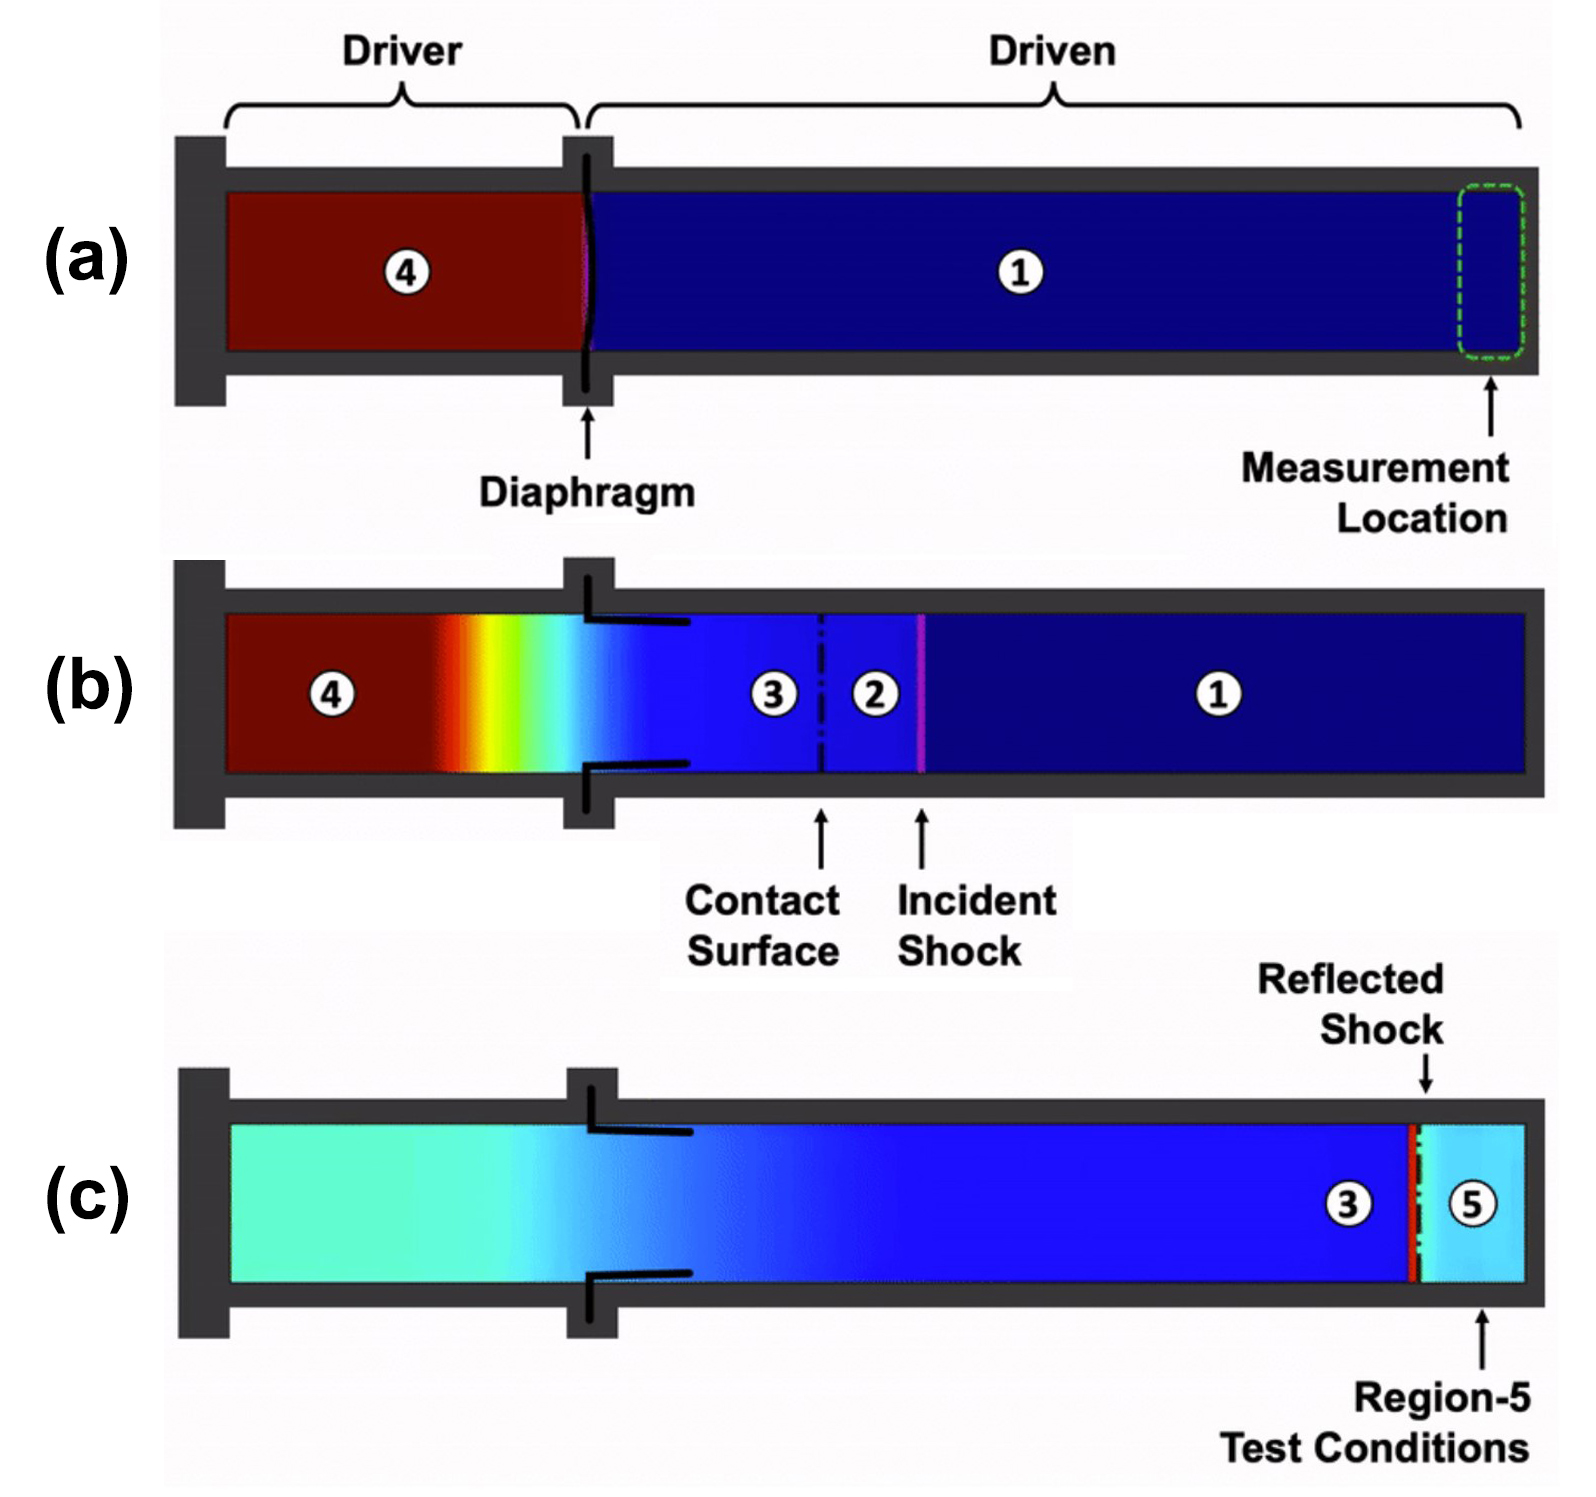
\includegraphics[height=80mm, ]{Figures/Results/Shocktube/shockwavestages.jpg}
	\caption{Different stages of shock wave propagation during shock-tube test from (a) before rupture of diaphragm leading to (b) propagation of incident shock towards the end of shock-tube and (c) its reflection from the end wall that increases pressure and temperature of test gas (Reprinted from Ref.~\citep{HansonGroupShockTube}}
	\label{fig:shockwave}
\end{figure}

Different stages of shock-wave propagation is illustrated in Fig.\ref{fig:shockwave}. A shock tube consists of a driver and a driven section separated by a single-use diaphragm. The driver section contains usually an inert gas with a low molecular weight such as He, and the driven section is filled with the studied test gas. The driver section is pressurized to the desired pressure until the rupture of the diaphragm that puts in direct contact the two regions with a large pressure difference. This creates a shock wave that propagates through the driven section causing a pressure and temperature jump in the test gas. 

After reaching the end wall, the shock wave reflects back towards the driver end of the shock-tube resulting in a secondary compression and heating of the mixture, and ultimately stagnating the test gas. In nearly 10 $\mathrm{\mu}$s, this shock-heating process can bring the test gas from room-temperature to temperatures upwards of 10,000 K, and pressures more than 1000 atm.



%Figure~\ref{fig:shocktubeschem} (left pane) illustrates the schematics of a shock-tube along with the idealized wave diagram. Shock-tubes are typically designed as a several meter long cylindrical tube separated by thin diaphragm into a smaller driver section filled a high pressure inert gas, and a longer driven section with diluted reactants. When the diaphragm is ruptured, the first shock wave propagates through the reactant mixture. The front shock compresses the reactants adiabatically raising the temperature and pressure throughout the shock-tube from $\mathrm{T_1}$, $\mathrm{P_1}$ to $\mathrm{T_2}$, $\mathrm{P_2}$. The passage of the reflected shock from the end wall heats up the reactants for the second time reaching $\mathrm{T_5}$, $\mathrm{P_5}$. Figure~\ref{fig:shocktubeschem} (right pane) shows the first and second jump in pressure due to the front and reflected shocks, respectively, and the variation in soot volume fraction during the pyrolysis of 0.03\% benzene in Ar. The reflected shock creates a nearly still mixture with a constant temperature and pressure (as shown in left pane of Figure~\ref{fig:shocktubeschem}) which provides an ideal condition for kinetic studies and rate constant investigations~\citep{kee2017chemically}. Therefore, the use of a shock tube provides a unique opportunity for investigating the kinetics of soot formation from fuels and at various temperatures, pressures and concentrations.

%\begin{figure}[!htbp]
%	\centering
%	\begin{subfigure}[t]{0.4\textwidth}
%		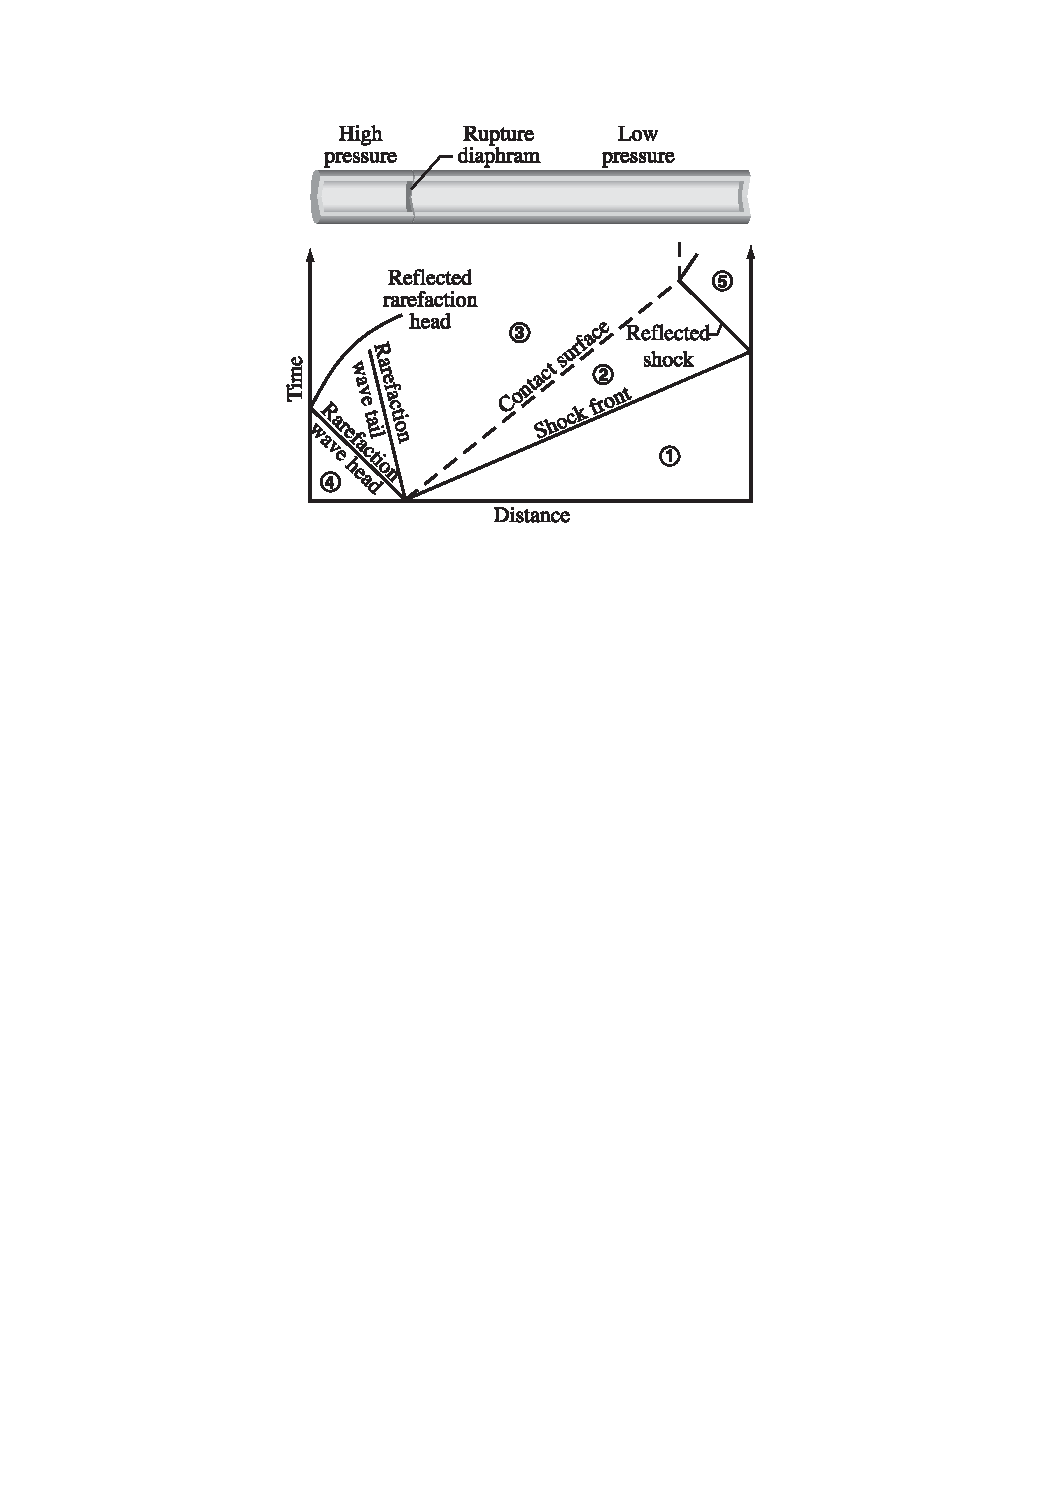
\includegraphics[width=1\textwidth]{Figures/Results/Shocktube/schematics.pdf}
%	\end{subfigure}
%	\begin{subfigure}[t]{0.4\textwidth}
%		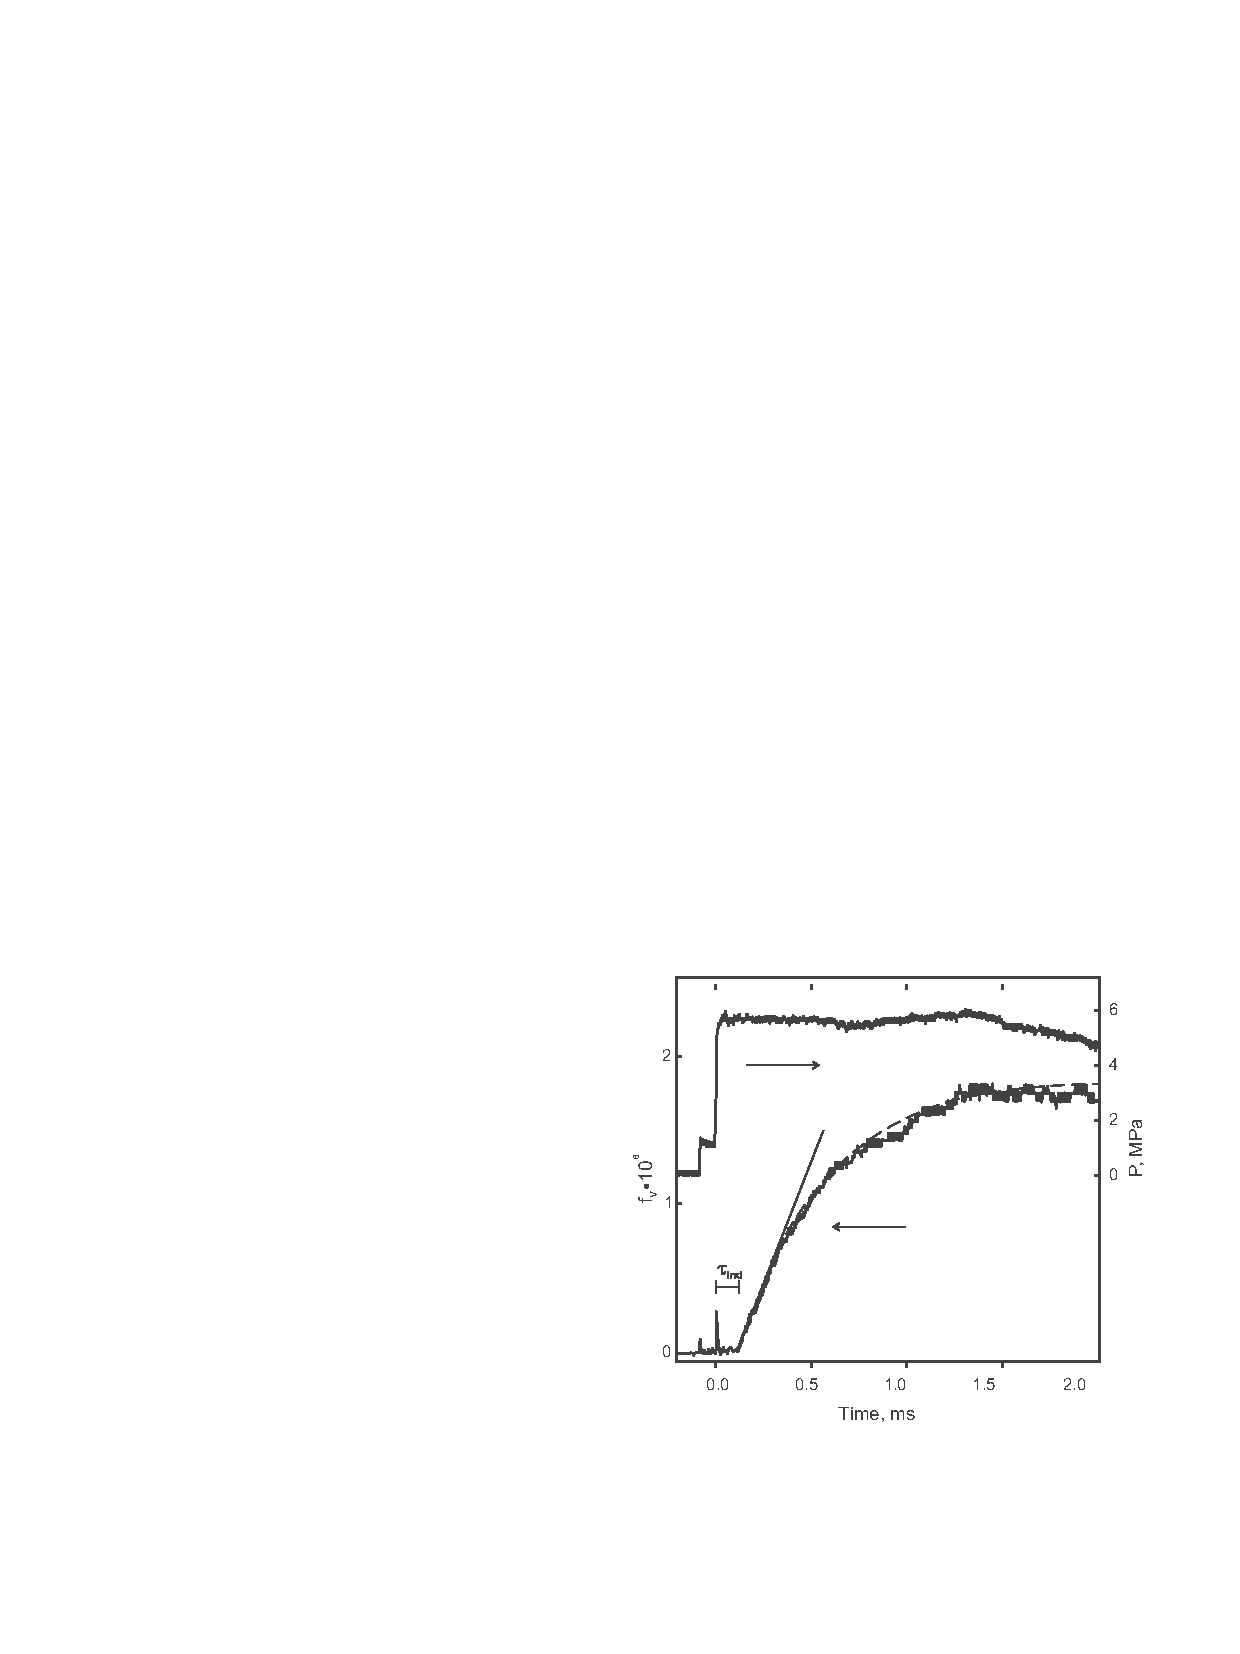
\includegraphics[width=1\textwidth]{Figures/Results/Shocktube/pfv_sample_shocktube.pdf}
%	\end{subfigure}
%	\caption{The schematics of a shock-tube and the idealized shockwave diagram(left pane reprinted from ~\citet{kee2017chemically}) and the variation of soot volume fraction measured by the extinction record at 633 nm and the pressure profile behind the reflected shock wave in a mixture 0.03\% benzene in Ar at T = 1890 K(right pane reprinted from ~\citet{karasevich1994soot})}
%	\label{fig:shocktubeschem}
%\end{figure}

The passage of reflected shock, referred to as region 5 with $\mathrm{T_5}$ and $\mathrm{P_5}$, is reference for calculation of residence time and the starting point for simulations. The delay in appearance of soot (often quantified by a threshold for LII or extinction signals) is know as induction time, $\mathrm{\tau_{ind}}$. There has been a lot of research in the literature focused on induction time (similarly on ignition delay time) in shock tubes~\citep{fussey1978shock}, but it is not the focus of this work. Instead, we mainly focus on  species concentrations and soot characteristics during the pyrolysis of methane, at atmospheric and higher pressure which can be used for the design and optimization of carbon black in plasma reactors~\citep{fulcheri2023energy}. 

%----------------------------------------------------------------
%
% STANFORD SHOKCTUBE DATA 30% CH4
%
%----------------------------------------------------------------

\subsection{Experimental setup and data collection}

The experiments on $\mathrm{CH_4}$ pyrolysis were conducted by Hanson Research Group at Stanford University. The data has not been published yet (at the time of writing the document) and were provided through the collaboration with Monolith Materials and Stanford University.

Mole fraction time histories of methane (CH4), acetylene (C2H2), and ethylene (C2H4) were captured using continuous wave (CW) laser absorption at 3.365 $\mu$m, 2.998 $\mu$m, and 10.532 $\mu$m, respectively~\citep{pinkowski2019multi, cassady2020thermal, stranic2014laser}. Soot volume fraction was measured using laser light extinction at $\lambda$=633 nm and 1064 nm with absorption function E(m) of 0.174 and 0.203~\citep{lee1981optical}, respectively. Additionally, soot samples were collected onto imaging stubs mounted in the shock-tube end-wall. A schematic of the experimental setup for laser diagnostics in the shock tube is shown in Fig.~\ref{fig:shocktubelaserlayout}. Samples were extracted from the interior surface of the shock tube endwall after each experiment to allow for imaging and analysis of the particulates. TEM images were recorded with a FEI Tecnai G2 F20 X-TWIN microscope and Gatan SC200 camera for the test case of $\mathrm{P_5}$=4.5 atm and $\mathrm{T_5}$=2217 K.

\begin{figure}[H]
	\centering
	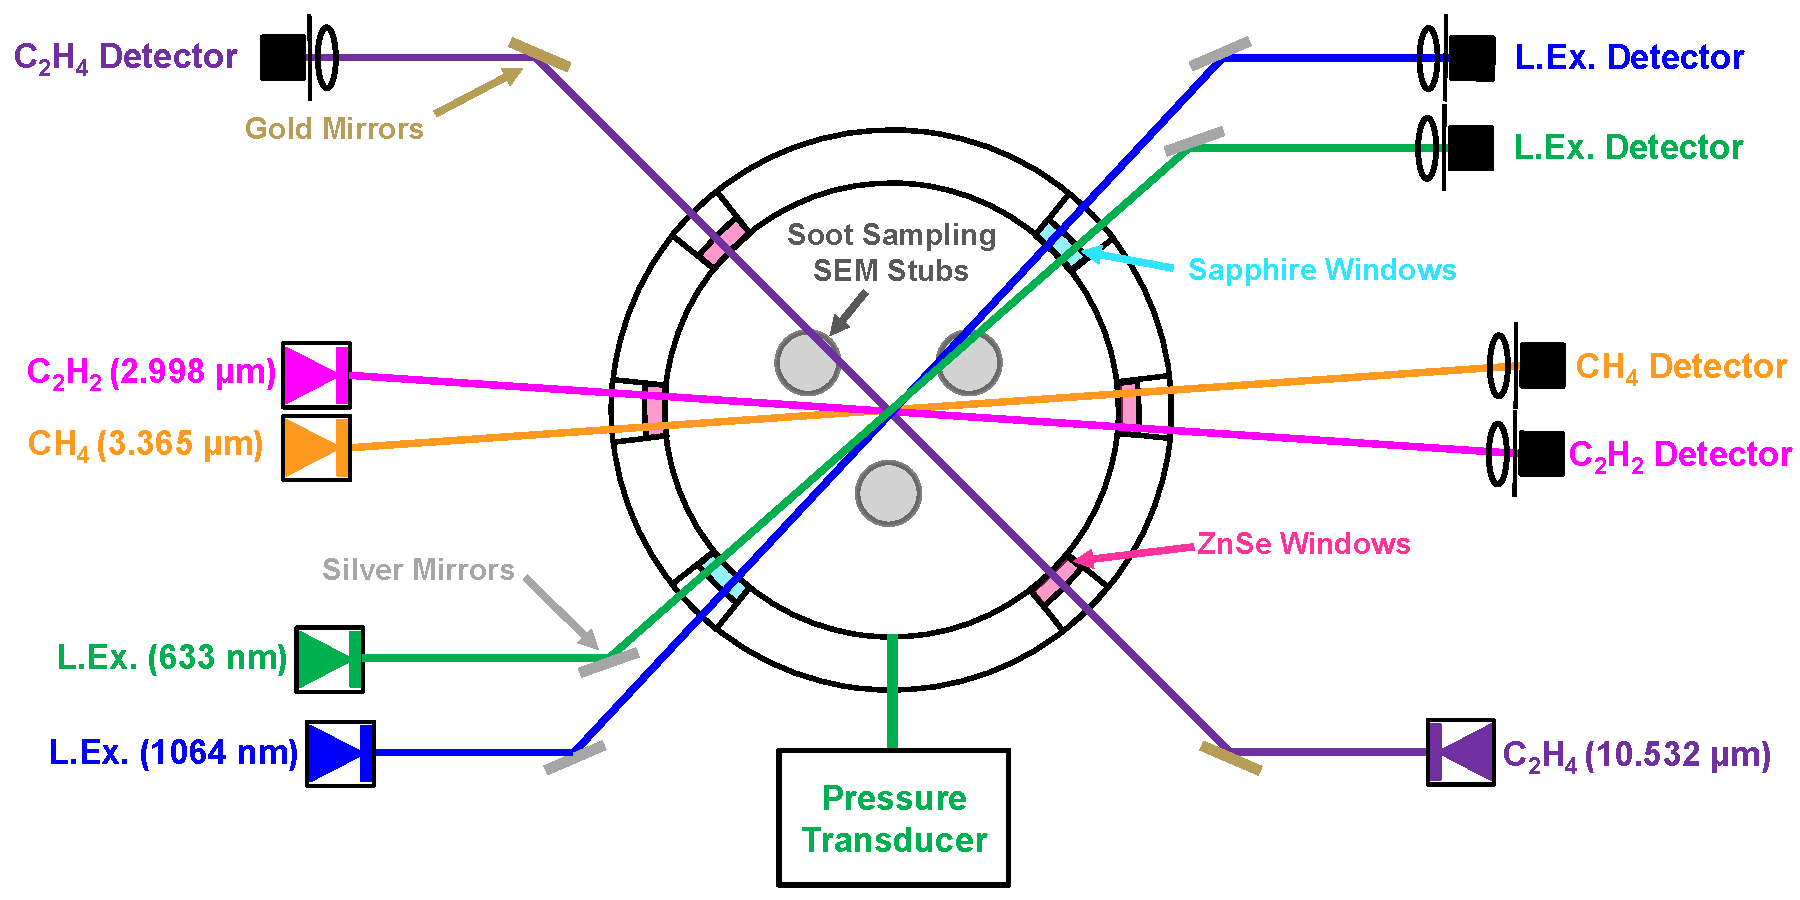
\includegraphics[width=0.75\textwidth]{Figures/Results/Shocktube/laserdiagnostics.pdf}
	\caption{Layout of the laser diagnostics and shock-tube setup. Spatial and spectral filtering is employed to ensure high-quality absorbance measurements to infer species mole fractions and soot volume fraction. Soot samples are collected at the shock-tube endwall. All lasers are aligned in a plane 1 cm from the endwall}
	\label{fig:shocktubelaserlayout} 
\end{figure}

The first data set includes eight measurements with the fuel loading of 30\% $\mathrm{CH_4}$-Ar at P=4$\pm$0.5 atm in the temperature range of 1800-2500 K. Table~\ref{tab:shocktubest_CH4_30} lists the process conditions including pressure, temperature and composition of all data points of 30\% $\mathrm{CH_4}$ pyrolysis.


\begin{table}[]
	\caption{The pressure, temperature and composition of simulation data points for 10\% $\mathrm{CH_4}$}
	\centering
	\begin{tabular}{l|llllllll|}
		\cline{2-9}
     	& \multicolumn{8}{c|}{Datapoints}                       \\ \cline{2-9} 
		& (1)  & (2)  & (3)  & (4)  & (5)  & (6)  & (7)  & (8)  \\ \hline
		\multicolumn{1}{|l|}{T {[}K{]}}   & 1861 & 1917 & 2030 & 2155 & 2184 & 2313 & 2375 & 2455 \\ \hline
		\multicolumn{1}{|l|}{P {[}atm{]}} & 4.12 & 3.74 & 3.56 & 3.93 & 3.62 & 3.58 & 3.75 & 3.47 \\ \hline
		\multicolumn{1}{|l|}{Composition} & \multicolumn{8}{c|}{$\mathrm{CH_4}$: 0.3, Ar: 0.7}               \\ \hline
	\end{tabular}
	\label{tab:shocktubest_CH4_30} 
\end{table}

 The time history of $\mathrm{CH_4}$, $\mathrm{C_2H_4}$ and $\mathrm{C_2H_2}$ mole fraction as well as soot yield and volume fraction were reported up to 0.5 ms. The constant volume reactor was used with all PAH growth and particle dynamics models. First, the performance of reaction mechanisms are assessed by comparing the mole fraction of species captured by laser diagnostics, $\mathrm{CH_4}$, $\mathrm{C_2H_4}$, and $\mathrm{C_2H_2}$ with model predictions using Caltech~\citep{blanquart2009chemical}, KAUST~\cite{wang2013pah} and ABF~\citep{appel2000kinetic} mechanisms. The analysis of simulation results (see Figs.~\ref{fig:shocktubest_30ch4_ch4_0}-\ref{fig:shocktubest_30ch4_ch4_0}) showed that soot formation described by different PAH growth and particle dynamcis models have negligible impact on prediction the mole fraction of measured species in the entire studied temperature range. Therefore, the assessment of reaction mechanisms for prediction of major species is performed without soot to simply the analysis. Figs.~\ref{fig:shocktubest_30ch4_ch4_nosoot_subset}-\ref{fig:shocktubest_30ch4_c2h2_nosoot_subset} compares the mole fraction of $\mathrm{CH_4}$, $\mathrm{C_2H_4}$, $\mathrm{C_2H_2}$ predicted by Caltech, KAUST, and ABF with data from laser diagnostics. Note that only a subset of simulations at T=1861, 2083, and 2375 K are shown for brevity. The species mole fraction for the whole temperature range is shown in Figs.~\ref{fig:shocktubest_30ch4_nosoot_ch4}-\ref{fig:shocktubest_30ch4_nosoot_c2h2}. $\mathrm{CH_4}$ mole fraction starts with a sharp drop from 0.5 at the beginning (corresponding to fast decomposition of methane) followed by a more gradual decrease. The initial decomposition rate increases with temperature. All mechanisms underpredict $\mathrm{CH_4}$ mole fraction, but ABF mechanism predictions are closer to the measurements than KAUST and Caltech. In other words, KAUST and Caltech overestimate $\mathrm{CH_4}$ conversion rate.
 %directing more carbon towards larger hydrocarbons and PAHs. 
 The mole fraction of $\mathrm{C_2H_4}$ (Fig.\ref{fig:shocktubest_30ch4_c2h4_nosoot_subset}) starts with a quick jumps after methane decomposition, reaches the maximum value and gradually decreases towards its final value. The simulations extended beyond test time of shock-tube calculations showed that $\mathrm{C_2H_4}$ mole fraction by KAUST and Caltech mechanisms continues to decrease to the equilibrium values, but ABF predicts a subsequent increase at longer residence times indicating reversal of $\mathrm{C_2H_4}$ decomposition which is more pronounced at high temperatures. The $\mathrm{C_2H_2}$ mole fraction increases in two steps, a rapid increase at the beginning followed by a gradual one. ABF mechanism predictions are in good agreement with measurements, but Caltech and KAUST underpredict the $\mathrm{C_2H_2}$ mole fraction. The difference between mechanisms are more pronounced at equilibrium. While ABF predicts a plateau beyond 1.5 ms, KAUST and Caltech predict a decrease towards a lower equilibrium value indicating conversion of acetylene to larger hydrocarbons and PAHs. The carbon mass fraction (CMF) of measured species, $\mathrm{CH_4}$, $\mathrm{C_2H_4}$ and $\mathrm{C_2H_2}$ combined is shown in Fig.~\ref{fig:shocktubest_30ch4_ccc_nosoot_subset}. The CMF of different mechanisms overlap decreasing up to a certain time that shortens with temperature. Beyond that, ABF mechanism predicts an increasing trend indicating that carbon returns to major species, but KAUST and Caltech continuously transfer carbon from measured species to larger hydrocarbons. This is consistent with the CMF of soot precursors shown in Fig.~\ref{fig:shocktubest_30ch4_spc_nosoot_subset}, which is significantly larger for KAUST and Caltech compared with ABF by three to two orders of magnitude, so it is expected that ABF mechanism cannot provide enough precursors for soot model to predict volume fraction comparable with measurements.  
 \begin{figure}[H]
 	\centering
 	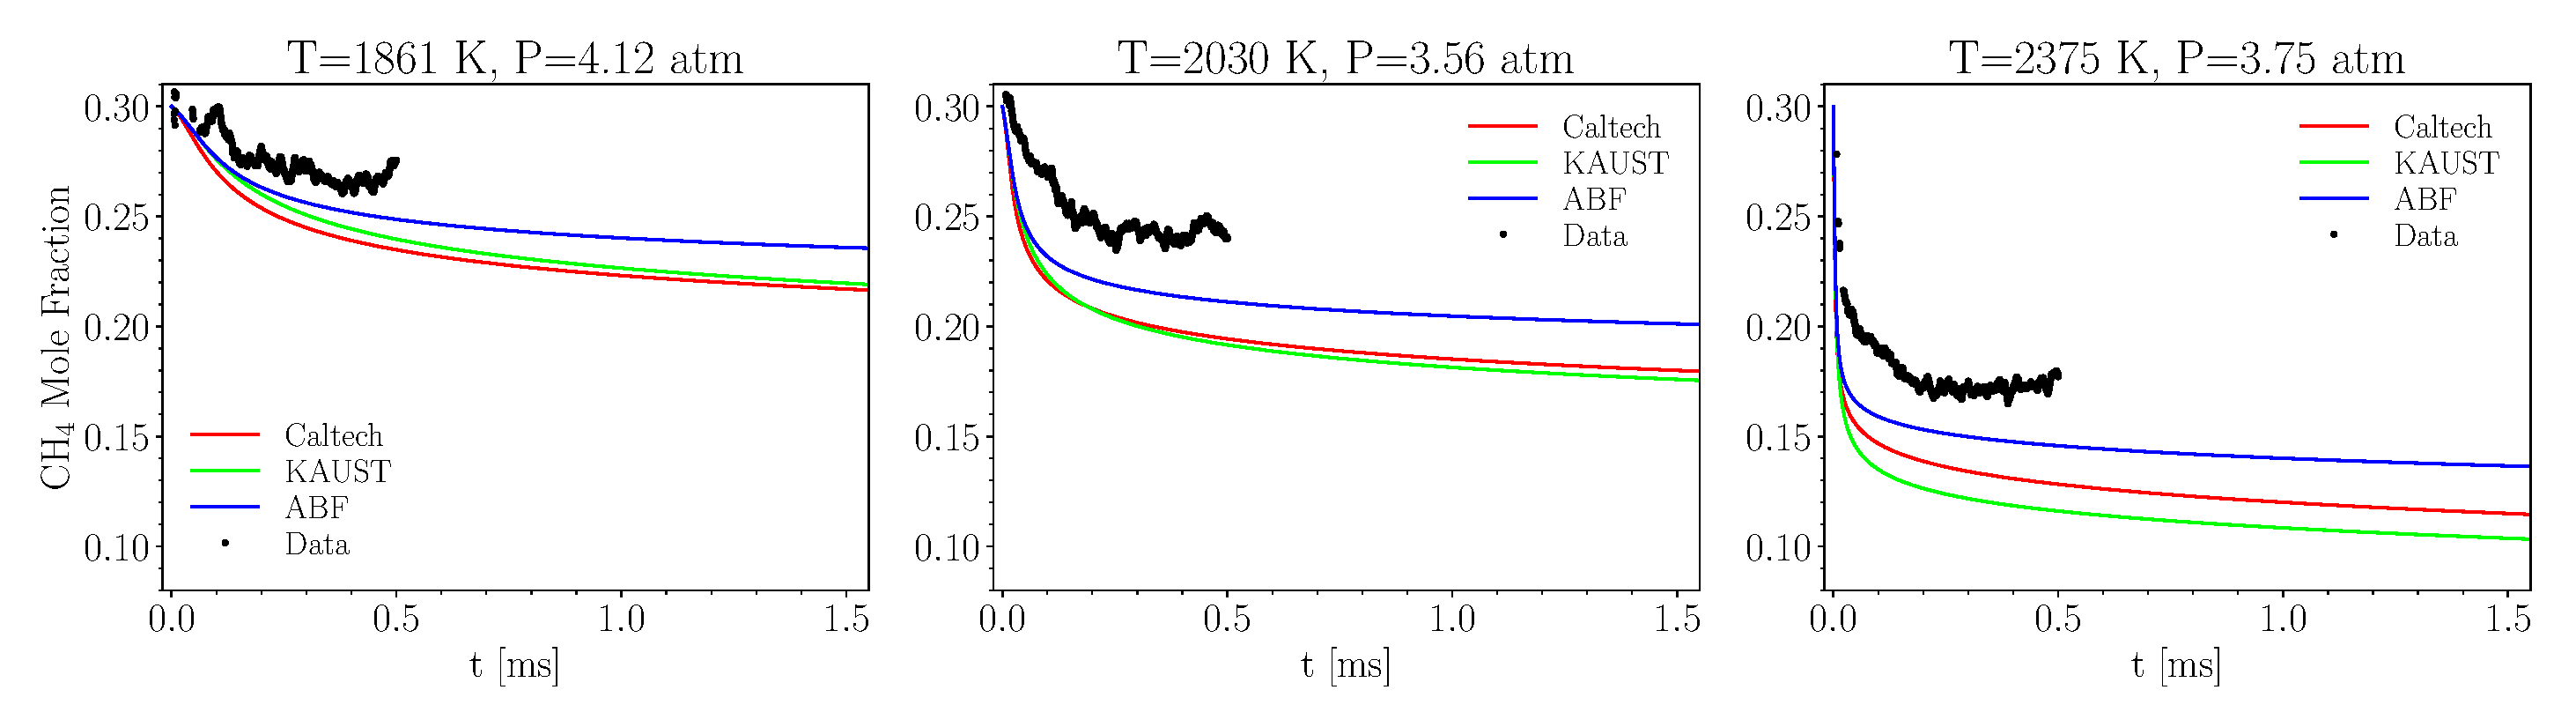
\includegraphics[width=1\textwidth]{Figures/Results/Shocktube/Stanford/june/30CH4_CH4_mechs_nosoot_subset.pdf}
 	\caption{The time history of carbon mass fraction of $\mathrm{CH_4}$ of 30\% $\mathrm{CH_4}$ pyrolysis at T=1861, 2083, and 2375 K using Caltech, KAUST, and ABF mechanisms compared with laser diagnostics data}
 	\label{fig:shocktubest_30ch4_ch4_nosoot_subset} 
 \end{figure}

 \begin{figure}[H]
	\centering
	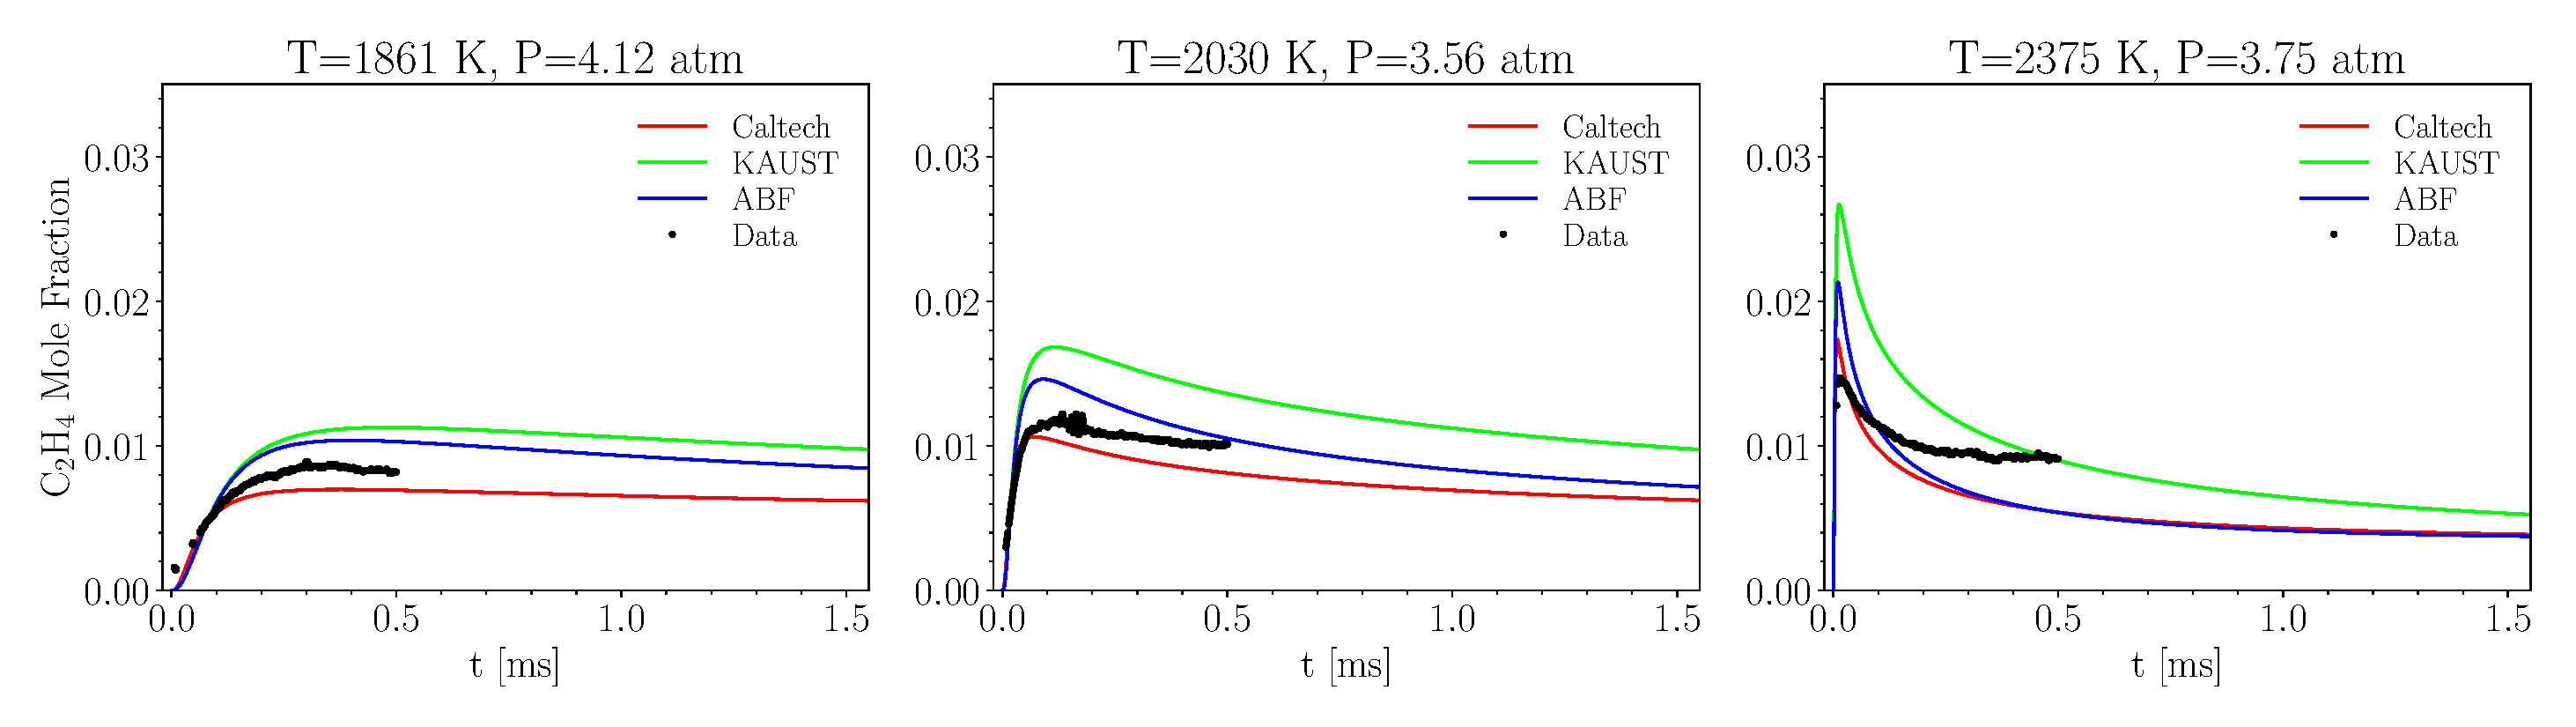
\includegraphics[width=1\textwidth]{Figures/Results/Shocktube/Stanford/june/30CH4_C2H4_mechs_nosoot_subset.pdf}
	\caption{The time history of carbon mass fraction of $\mathrm{C_2H_4}$ of 30\% $\mathrm{CH_4}$ pyrolysis at T=1861, 2083, and 2375 K using Caltech, KAUST, and ABF mechanisms compared with laser diagnostics data}
	\label{fig:shocktubest_30ch4_c2h4_nosoot_subset} 
\end{figure}

 \begin{figure}[H]
	\centering
	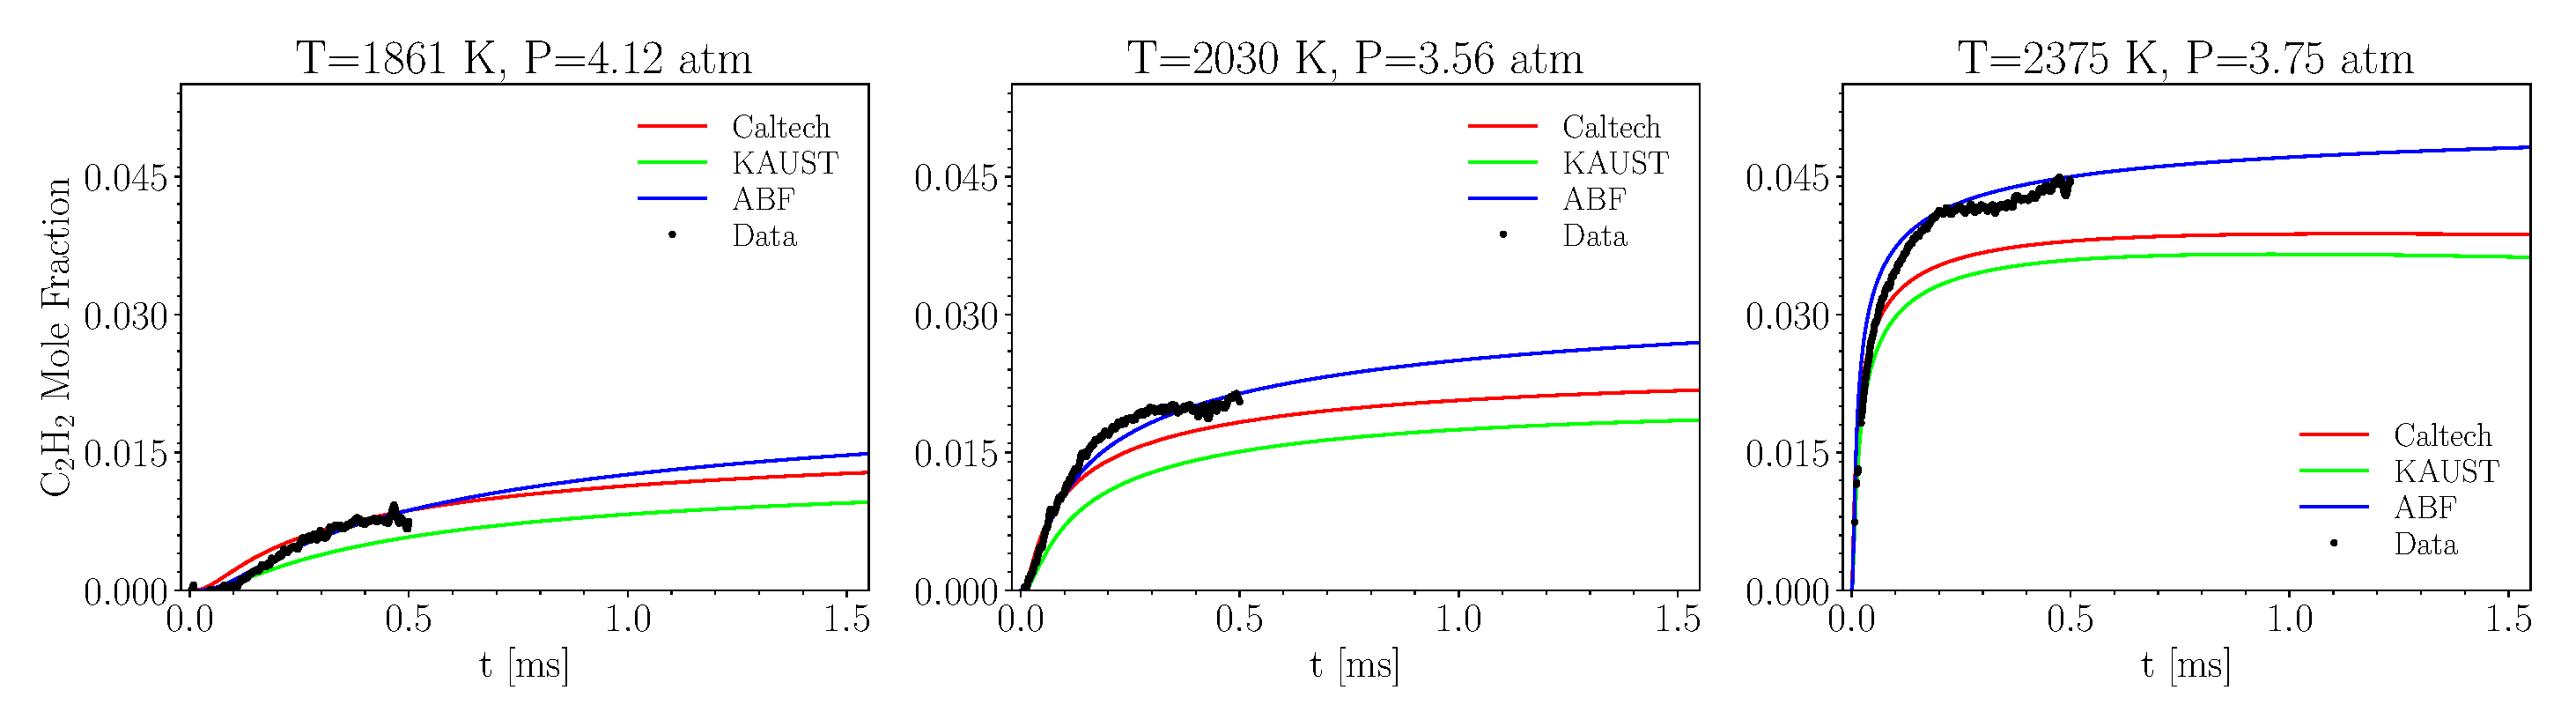
\includegraphics[width=1\textwidth]{Figures/Results/Shocktube/Stanford/june/30CH4_C2H2_mechs_nosoot_subset.pdf}
	\caption{The time history of carbon mass fraction of $\mathrm{C_2H_2}$ of 30\% $\mathrm{CH_4}$ pyrolysis at T=1861, 2083, and 2375 K using Caltech, KAUST, and ABF mechanisms compared with laser diagnostics data}
	\label{fig:shocktubest_30ch4_c2h2_nosoot_subset} 
\end{figure}
 
 
\begin{figure}[H]
	\centering
	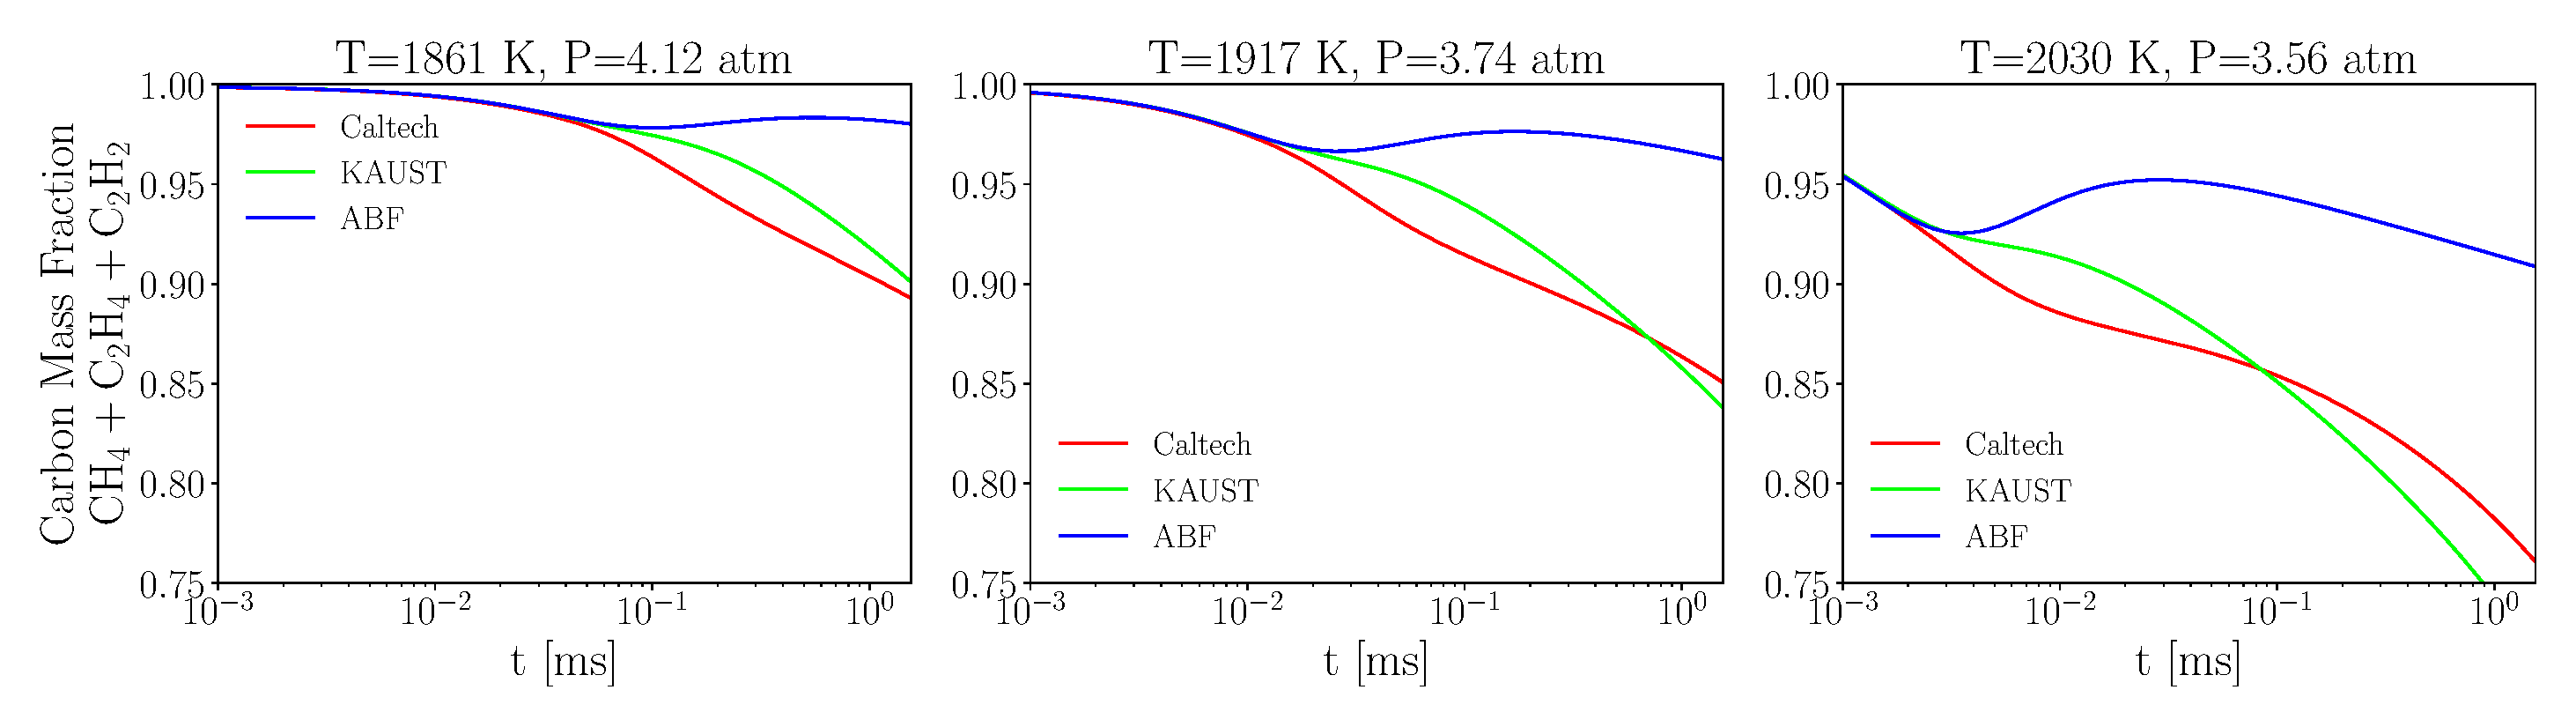
\includegraphics[width=1\textwidth]{Figures/Results/Shocktube/Stanford/june/30CH4_CCC_mechs_nosoot_subset.pdf}
	\caption{The time history of carbon mass fraction of $\mathrm{CH_4}$, $\mathrm{C_2H_4}$, $\mathrm{C_2H_2}$ of 30\% $\mathrm{CH_4}$ pyrolysis at T=1861, 2083, and 2375 K using Caltech, KAUST, and ABF}
	\label{fig:shocktubest_30ch4_ccc_nosoot_subset} 
\end{figure}
 

\begin{figure}[H]
	\centering
	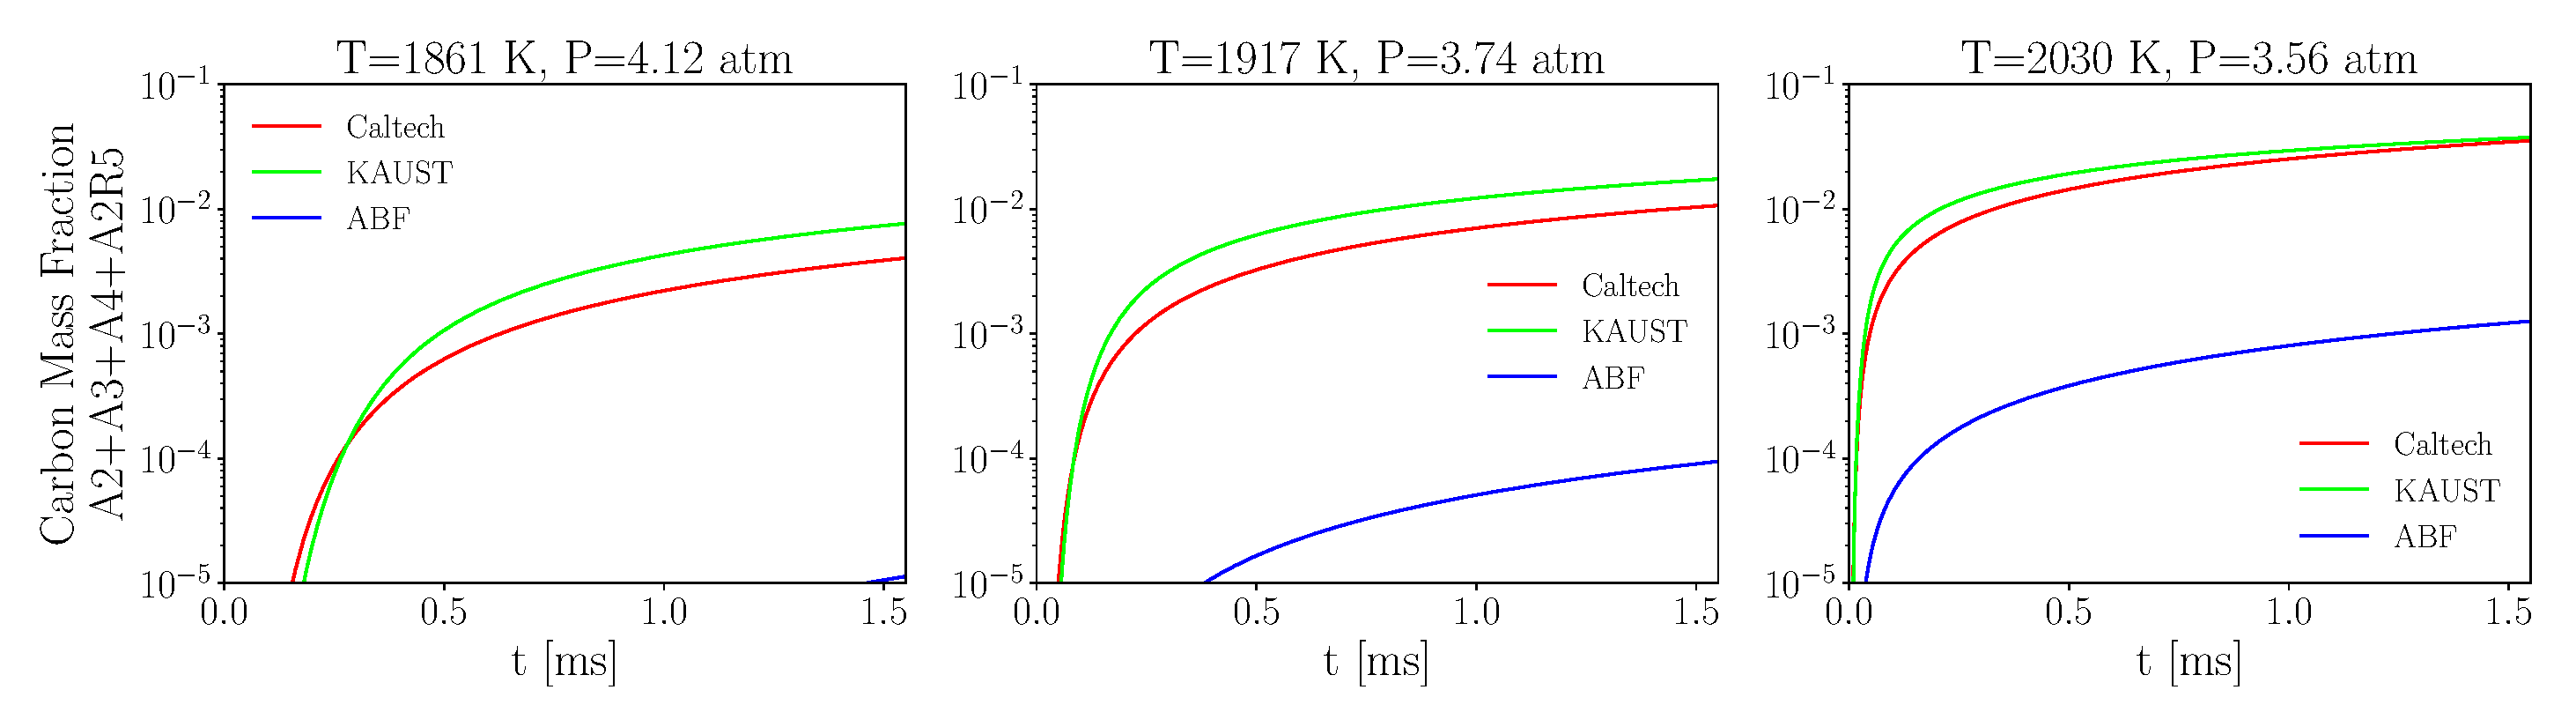
\includegraphics[width=1\textwidth]{Figures/Results/Shocktube/Stanford/june/30CH4_SPC_mechs_nosoot_subset.pdf}
	\caption{The time history of carbon mass fraction of soot precursors, A2, A3, A4 and A2R5 of 30\% $\mathrm{CH_4}$ pyrolysis at T=1861, 2083, and 2375 K using Caltech, KAUST, and ABF mechanisms}
	\label{fig:shocktubest_30ch4_spc_nosoot_subset} 
\end{figure}

Comparing $f_v$ predicted by three reaction mechanisms at T=2375 K and P=3.75 atm with the data from extinction measurements confirms the above-mentioned conclusion. As shown in Fig.~\ref{fig:shocktubest_30ch4_sootvf_single}, the $f_v$ by ABF follows a similar trend as data, but the values are nearly two orders of magnitude lower indicating small PAH concentrations. Although both Caltech and KAUST predict $f_v$ comparable with data, KAUST will be used for detailed soot simulations as its combination with E-Bridge Modified accurately captures soot volume fraction. Having said that, any conclusions drawn using KASUT can be generalized to Caltech as well.


\begin{figure}[H]
	\centering
	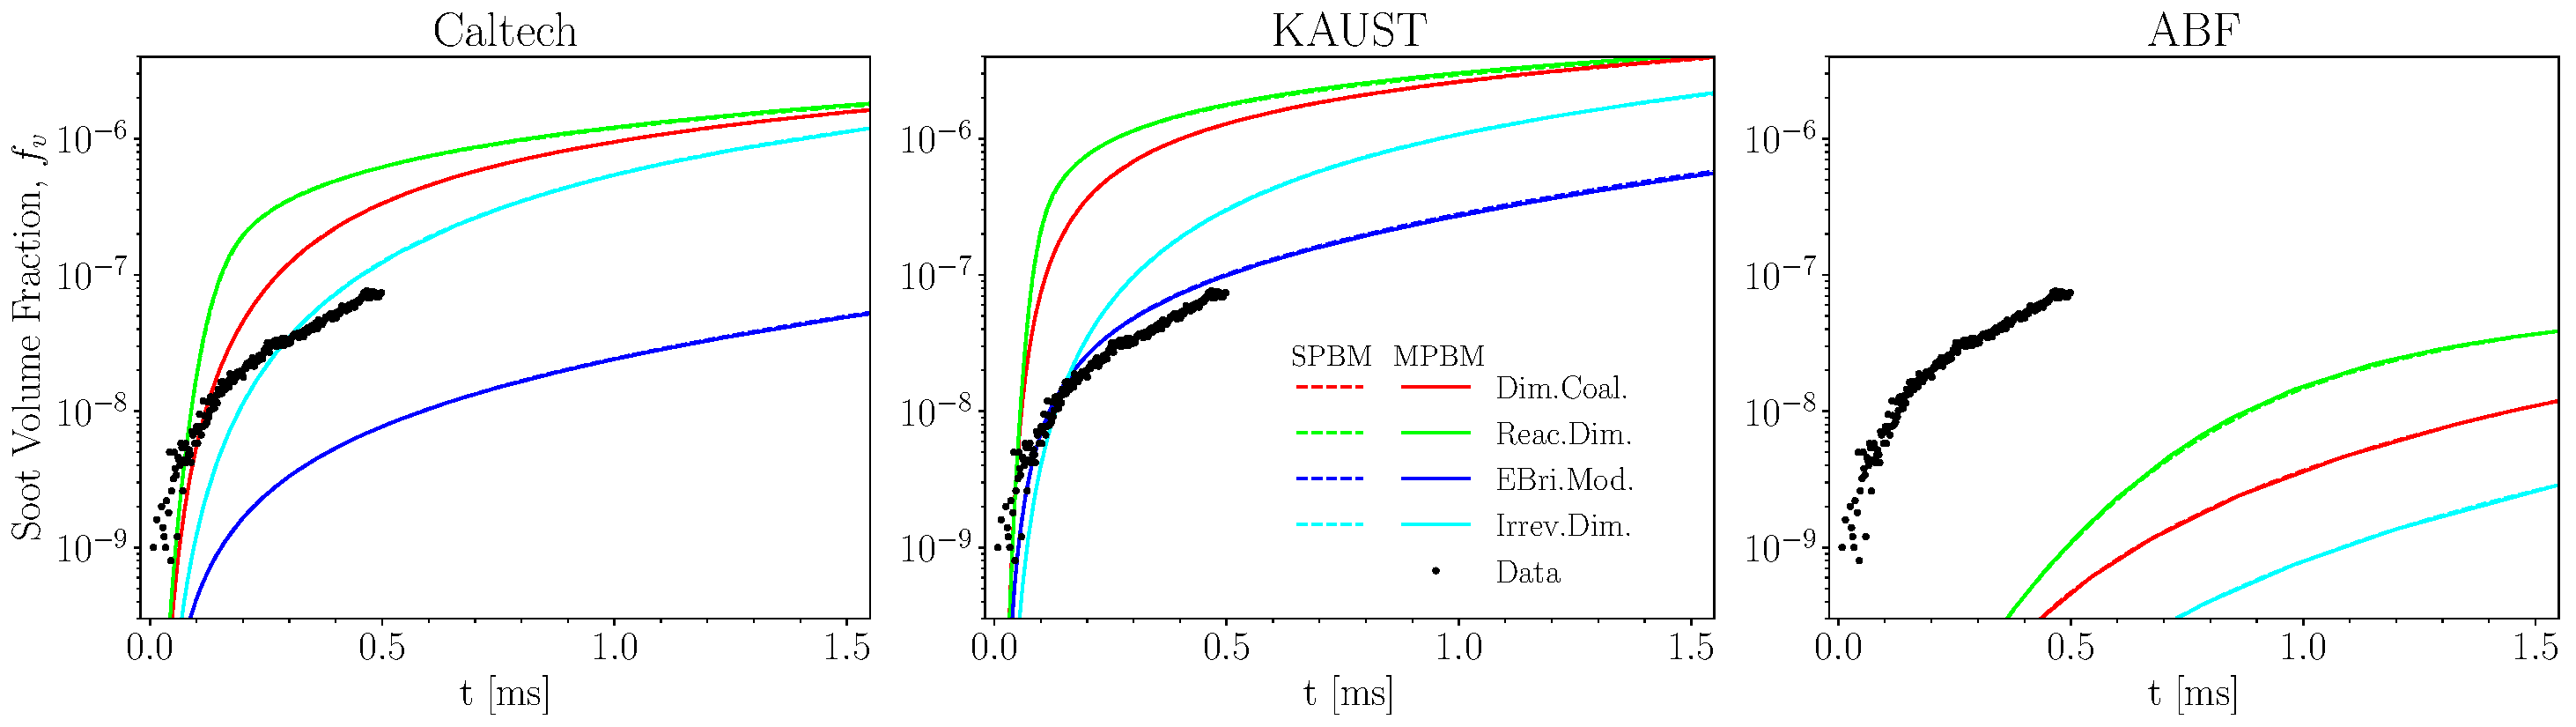
\includegraphics[width=1\textwidth]{Figures/Results/Shocktube/Stanford/june/30CH4_sootvf_mechs_single.pdf}
	\caption{The time history of soot volume fraction of 30\% $\mathrm{CH_4}$ pyrolysis at T=2375 K and P=3.75 atm using Caltech, KAUST, and ABF mechanism and different PAH growth and particle dynamics models}
	\label{fig:shocktubest_30ch4_sootvf_single} 
\end{figure}

Fig.~\ref{fig:shocktubestcasevf} shows that the time variation of soot volume fraction in the temperature range of 1800-2500 K. The measurement data was not available (or too noisy) below T=2155 K due to lack of enough soot particle leading to weak extinction signal. In all cases with higher temperatures, EBridge Formation predicts the lowest volume fraction that interestingly are in close agreement with the data. Reactive Dimerization and Dimer Coalescence yields the largest $f_v$ nearly two orders of magnitude higher than the measurements that start with a rapid increase indicating a stronger inception rate leading to larger number concentration of particles that provide more surface area for surface growth via HACA. Shock tube temperature increases $f_v$ with all PAH growth models over the 1.5 ms. Moreover, high temperature accelerates soot formation, which can be examined by comparing $f_v$ at early stages of simulation. For example, no soot appears before t=0.25 ms i.e. $f_v<10^{-10}$ at T=1861 K, but $f_v$ approaches $10^{-6}$ at T=2455.

Fig.\ref{fig:shocktubestcasedp} shows the time history of primary particle diameter, $d_p$ at different temperatures. As expected, EBridge Formation and Irreversible Dimerization has the lowest $d_p$ due to low soot mass growth rate leading to small $f_v$ values. Although Dimer Coalescence and Reactive Dimerization generate close volume fraction values corresponding to similar soot mass, the latter predicts larger $d_p$ indicating a lower number of $N_{pri}$. In other words, RD has lower inception rates and a stronger PAH adsorption rate compared to DC. The $d_p$ by RD exhibits a noticeable sensitivity to particle dynamics model that grows with temperature. Both model predict the initial rapid rise in $d_p$. While MPBM predicts a gradual increase to final value, $d_p$ by SPBM decreases for T$>$2000 K due to stronger inception rate by SPBM that generates particle with $d_p$=2 nm bringing down the average $d_p$.

% Final fv in terms of temperature
% the time that it taks for each PAH growth model to each 50%/90% of the final value

\begin{figure}[H]
	\centering
	\includegraphics[width=1\textwidth]{Figures/Results/Shocktube/Stanford/june/stsh_cases_vf.pdf}
	\caption{The time history of soot volume fraction of 30\% $\mathrm{CH_4}$ pyrolysis in the temperature range of 1800-2500 K and P=4$\pm$0.5 atm using KAUST mechanism and different PAH growth and particle dynamics models}
	\label{fig:shocktubestcasevf} 
\end{figure}


\begin{figure}[H]
	\centering
	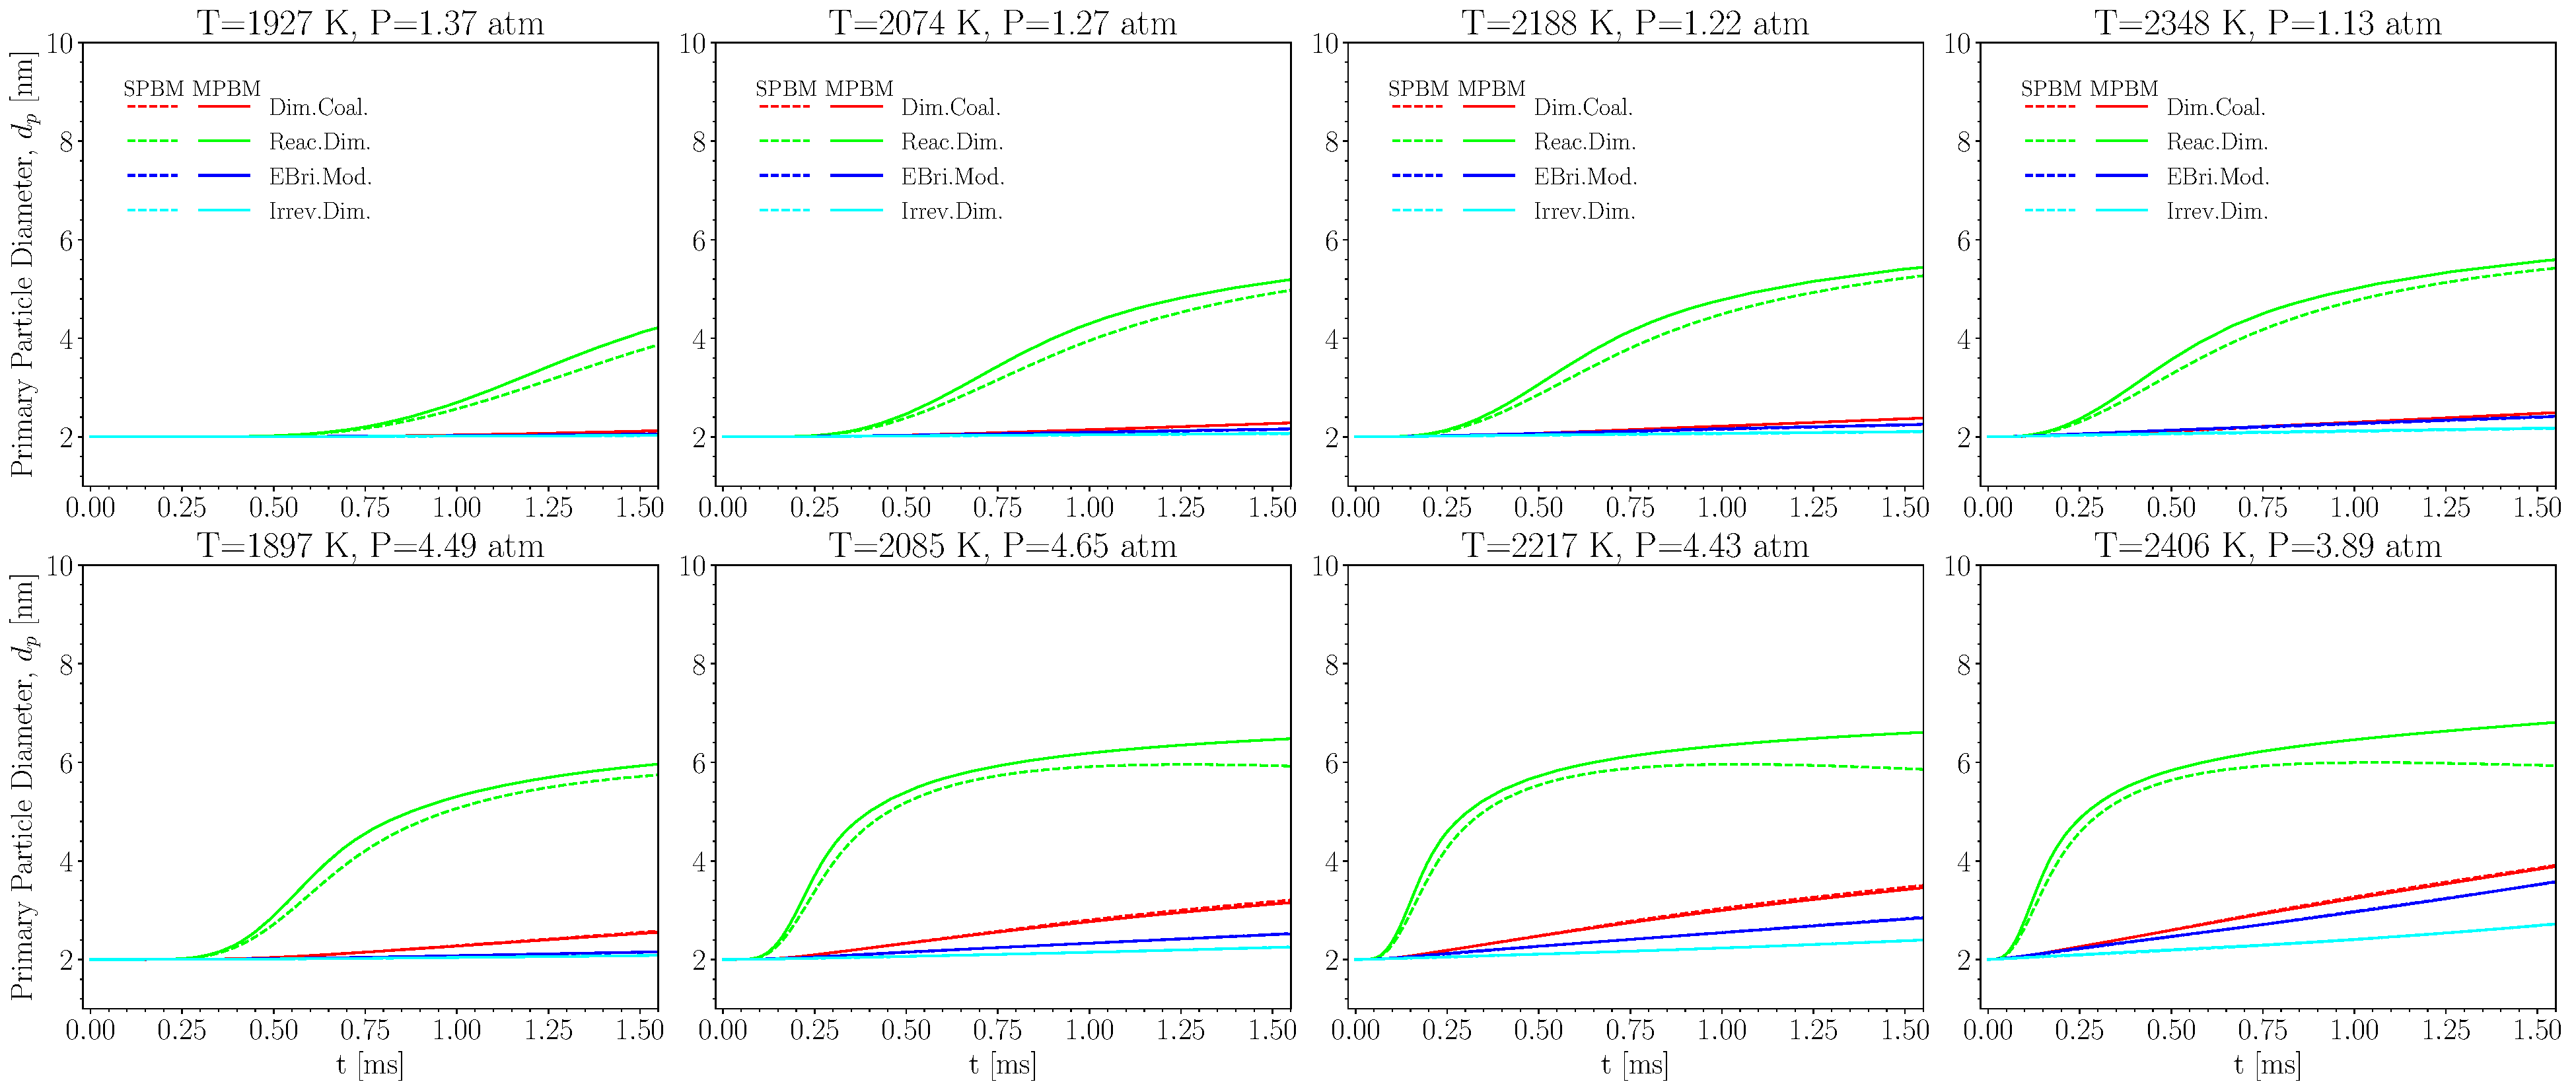
\includegraphics[width=1\textwidth]{Figures/Results/Shocktube/Stanford/june/stsh_cases_dp.pdf}
	\caption{The time history of primary particle diameter, $d_p$ of 30\% $\mathrm{CH_4}$ pyrolysis in the temperature range of 1800-2500 K and P=4$\pm$0.5 atm using KAUST mechanism and different PAH growth and particle dynamics models}
	\label{fig:shocktubestcasedp} 
\end{figure}

Fig.\ref{fig:shocktubestcasedm} shows time histories $d_m$ at different shock tube temperature. Similar to $d_p$, $d_m$ increases over time and with shock tube temperature. The rise in $d_m$ occurs faster. Initially, the generated agglomerates are small ($n_p\approx1$), and $d_m$ is close to $d_p$, so RD yield the highest $d_m$, but DC takes over and exceeds RD. Additionally, $d_m$ predicted by MPBM is larger in the beginning of the simulation, but $d_m$ predicted by SPBM rises faster at longer residence times. Fig.~\ref{fig:shocktubecarbon} shows the carbon mass growth rate by inception, HACA and PAH adsorption at T=2455 K and P=3.47 atm that explains the difference in the behavior of PAH growth and particle dynamics model in prediction of soot mass and morphology. The inception rate of RD (Fig.~\ref{fig:shocktubecarbon}-a) rapidly rises reaching its peak values and quickly drops until t=0.25 ms when a bifurcation occurs. While the inception rate by MPBM gradually decreases, SPBM predicts an increasing rate of production of new particles leading to a smaller $d_p$. DC reaches the inception peak higher than other PAH growth models before t=0.25 ms creating more particles that causes larger $d_m$ after coagulation becomes dominant. Such a high number concentration also leads to large HACA growth rates evident in Fig.~\ref{fig:shocktubecarbon}-b. RD has the highest PAH adsorption rate with a peak near t=0.1 ms as opposed to other PAH growth models that causes the rapid drop in inception rate and higher soot mass gain rates leading to larger volume fraction (Fig.\ref{fig:shocktubestvf}).

\begin{figure}[H]
	\centering
	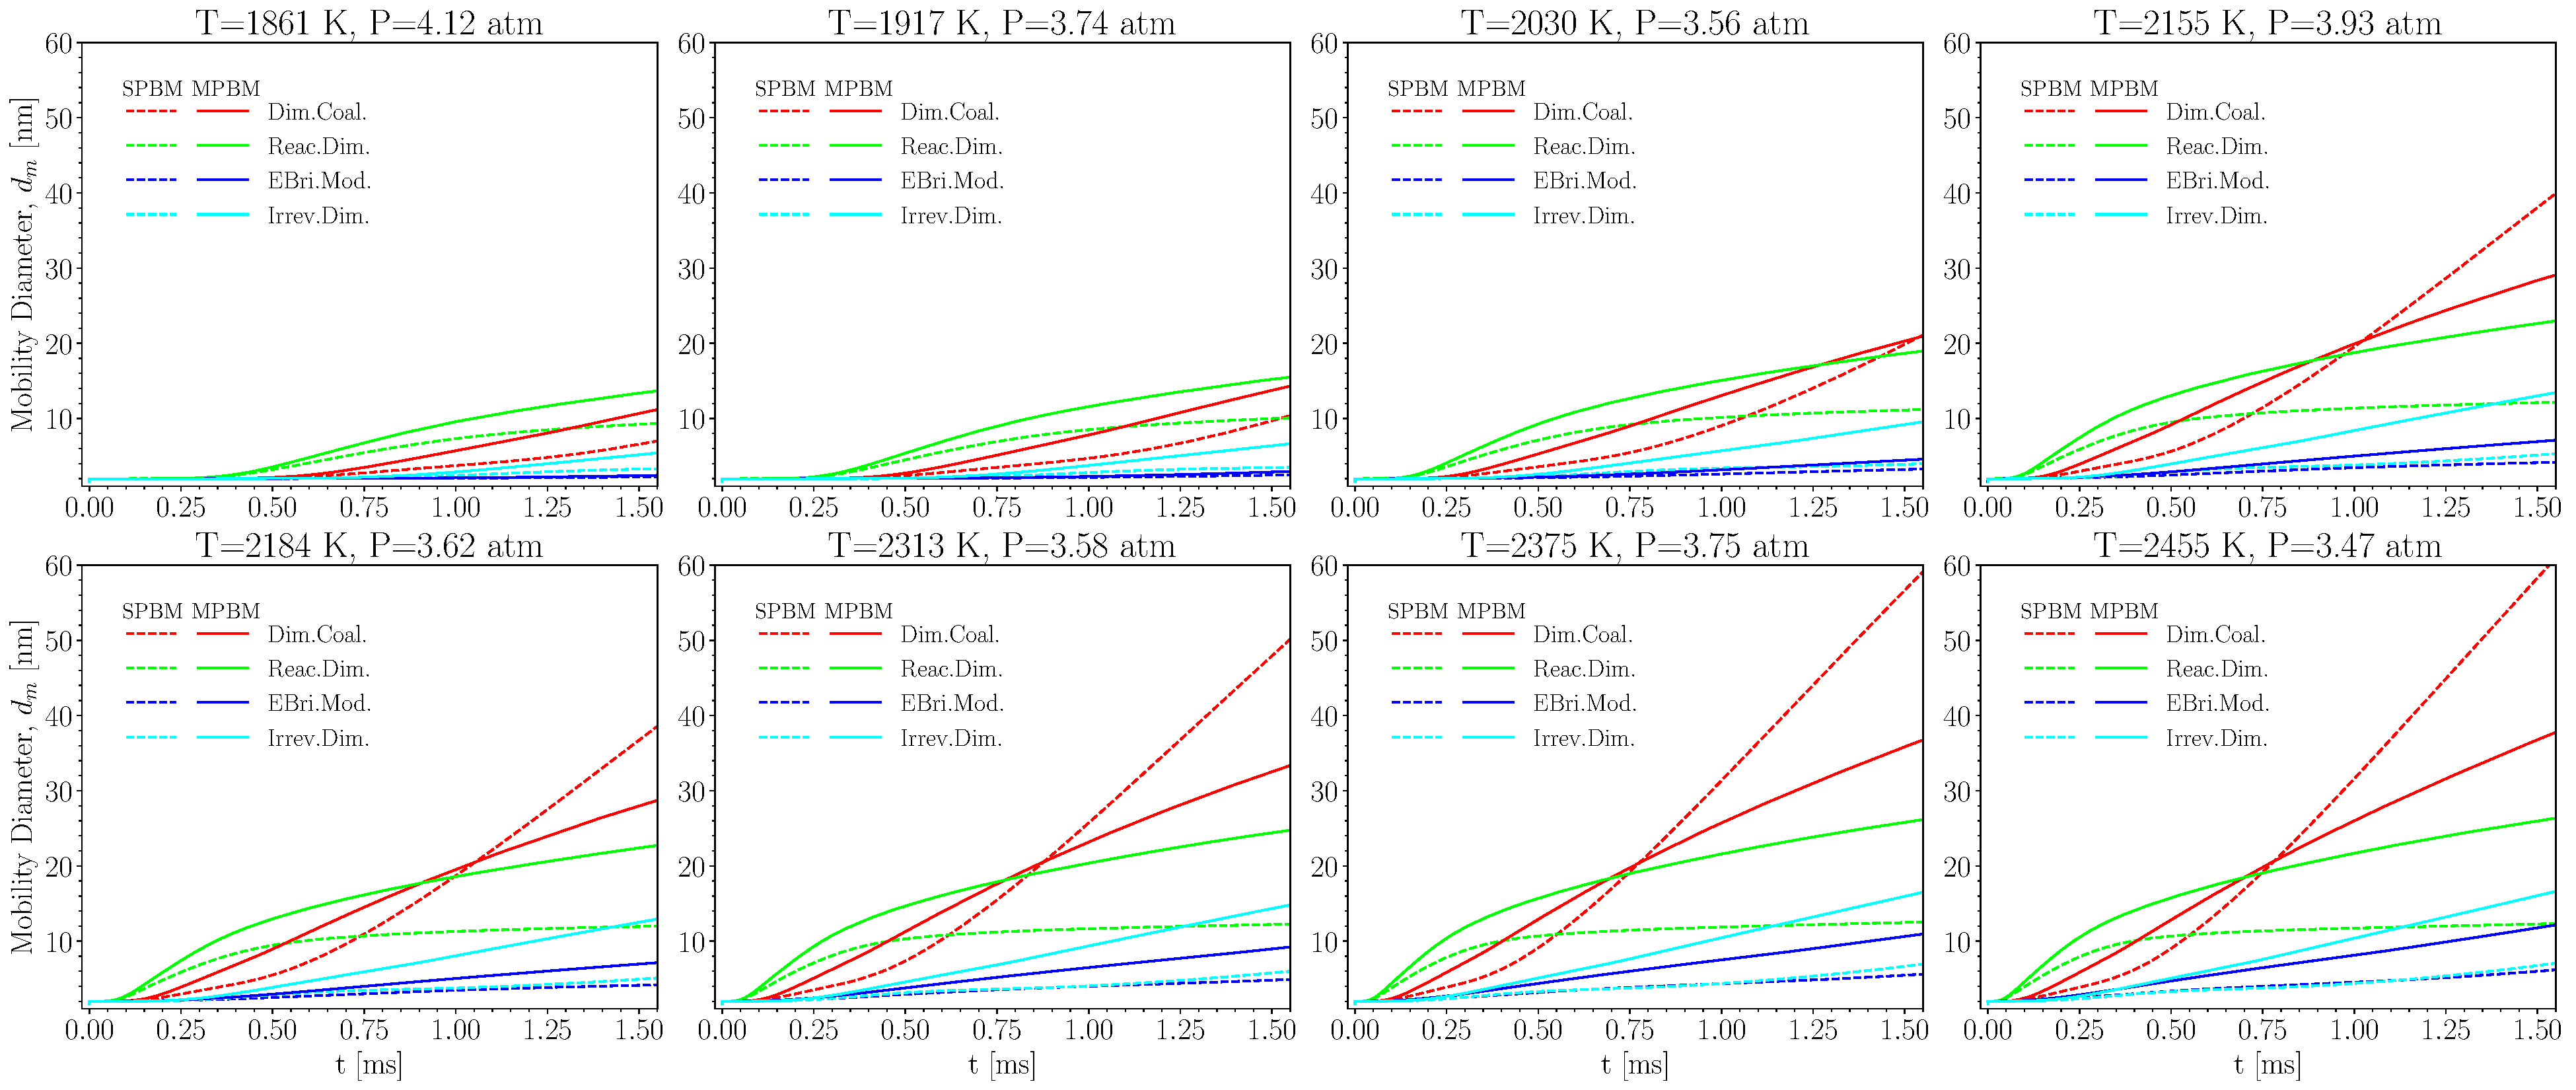
\includegraphics[width=1\textwidth]{Figures/Results/Shocktube/Stanford/june/stsh_cases_dm.pdf}
	\caption{The time history of mobility diameter, $d_m$ of 30\% $\mathrm{CH_4}$ pyrolysis in the temperature range of 1800-2500 K and P=4$\pm$0.5 atm using KAUST mechanism and different PAH growth and particle dynamics models}
	\label{fig:shocktubestcasedm} 
\end{figure}

\begin{comment}
	\begin{figure}[H]
		\centering
		\begin{subfigure}[t]{0.32\textwidth}
			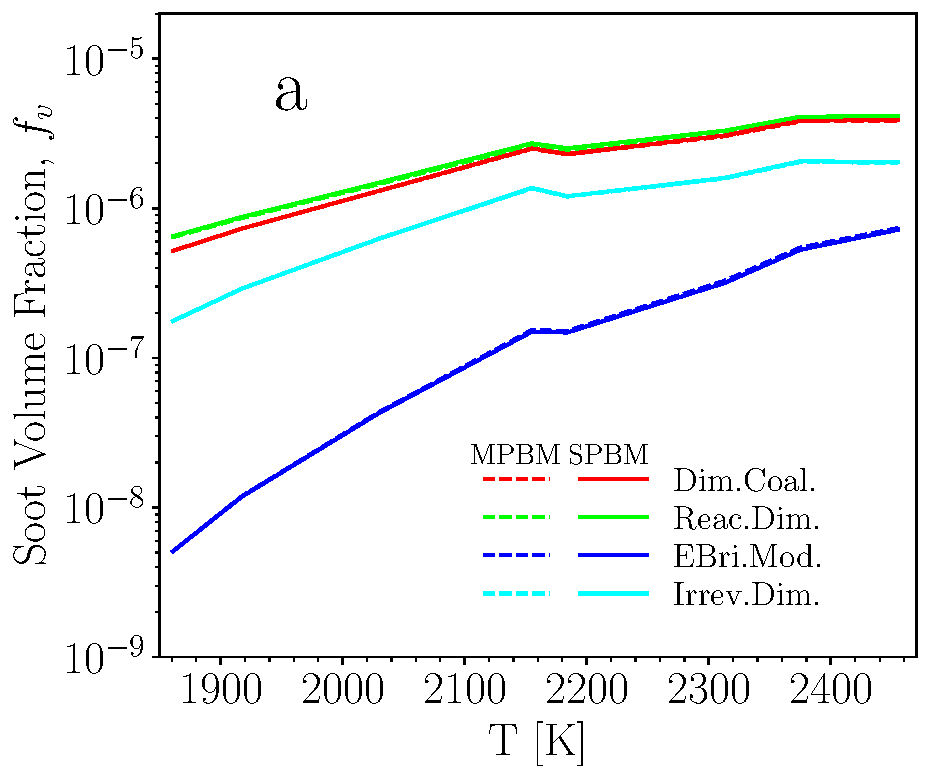
\includegraphics[width=1\textwidth]{Figures/Results/Shocktube/Stanford/June/stsh_temp_fv.pdf}
		\end{subfigure}
		\begin{subfigure}[t]{0.32\textwidth}
			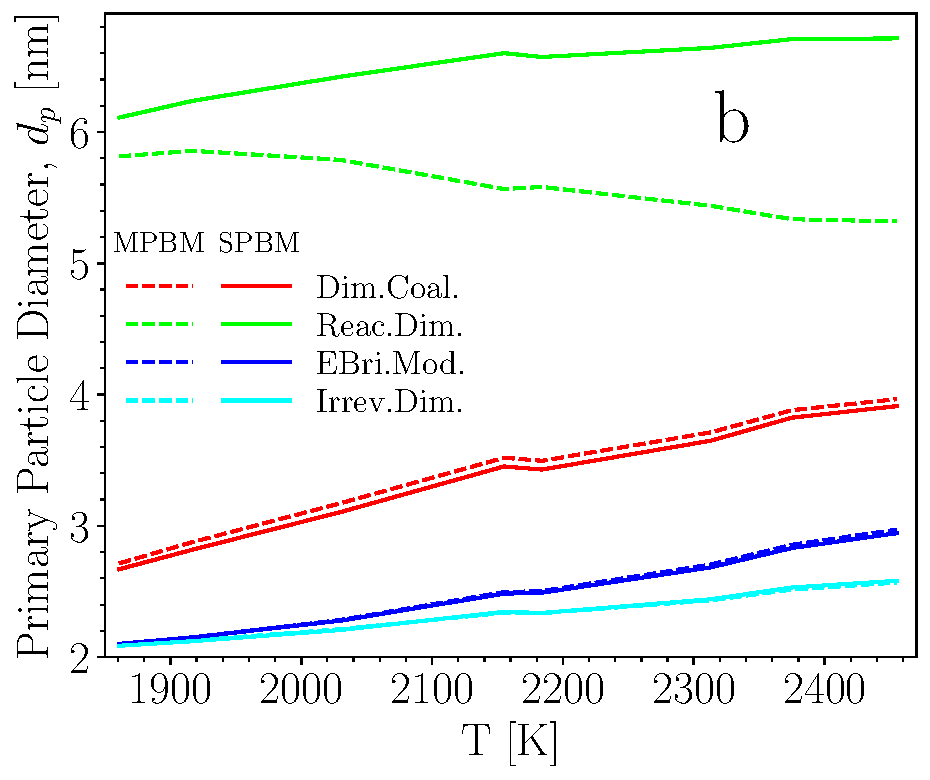
\includegraphics[width=1\textwidth]{Figures/Results/Shocktube/Stanford/June/stsh_temp_dp.pdf}
		\end{subfigure}
		\begin{subfigure}[t]{0.32\textwidth}
			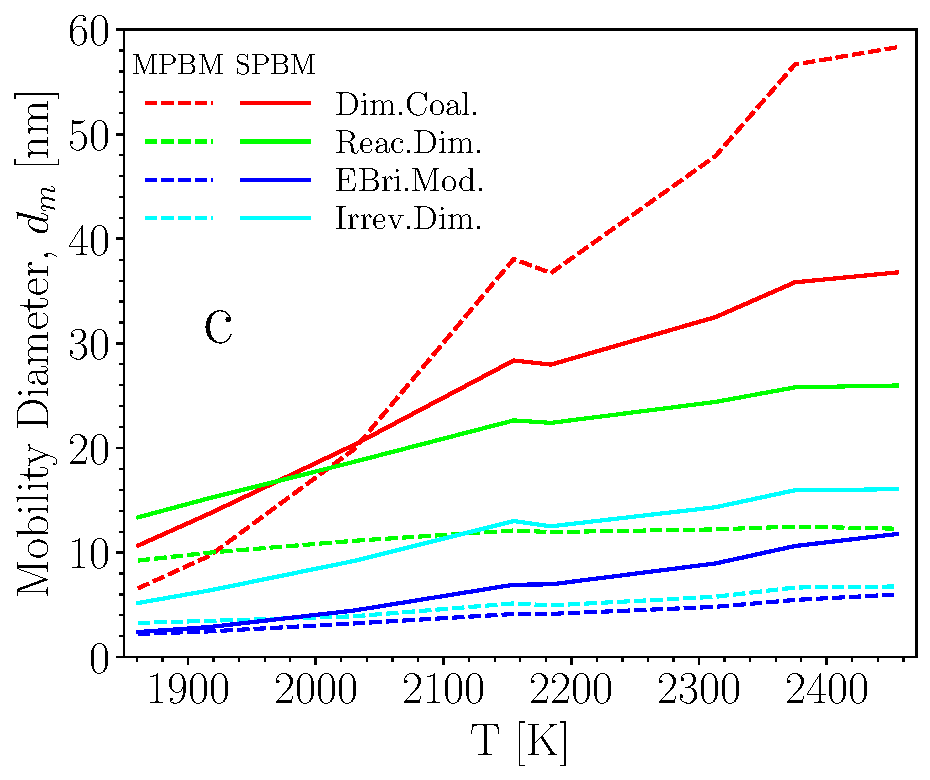
\includegraphics[width=1\textwidth]{Figures/Results/Shocktube/Stanford/June/stsh_temp_dm.pdf}
		\end{subfigure}
		\caption{The temperature dependence of volume fraction, $f_v$ (a), primary particle diameter, $d_p$ (b), mobility diameter, $d_m$ (c) at t=1.5ms of pyrolysis of 30\% $\mathrm{CH_4}$ in the temperature range of 1800-2500 K and P=4$\pm$0.5 atm using KAUST mechanism and different PAH growth and particle dynamics models}
		\label{fig:shocktubetemponehalf} 
	\end{figure}
\end{comment}



\begin{figure}[H]
	\centering
	\begin{subfigure}[t]{0.32\textwidth}
		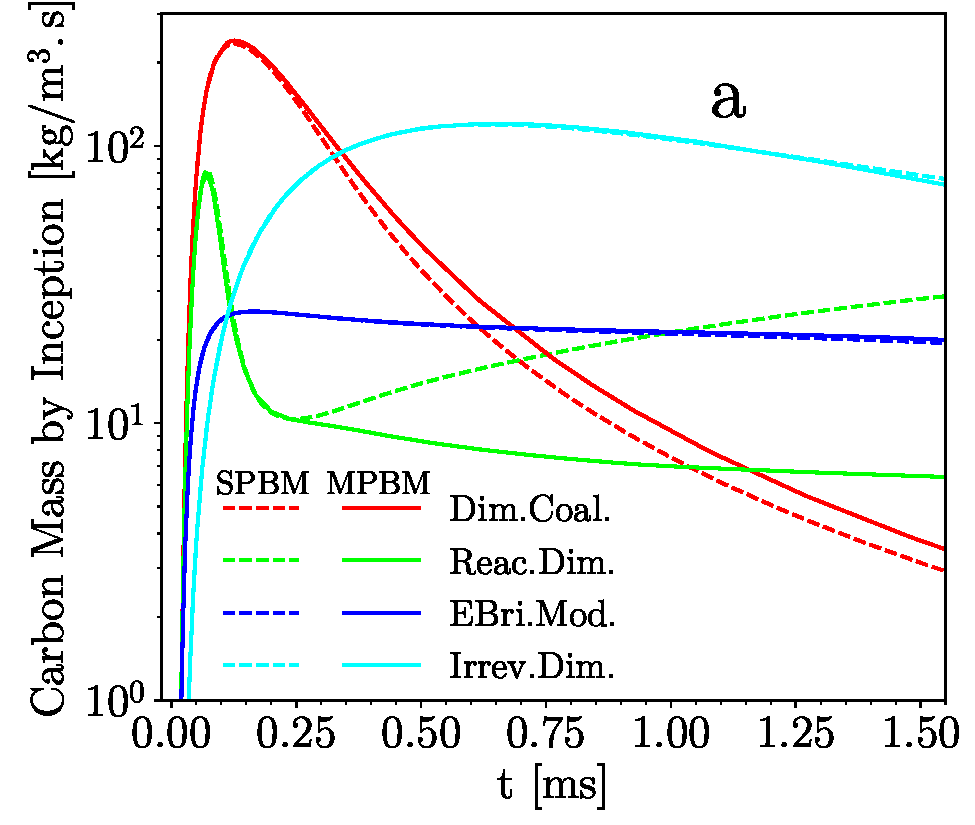
\includegraphics[width=1\textwidth]{Figures/Results/Shocktube/Stanford/June/stsh_single_inc.pdf}
	\end{subfigure}
	\begin{subfigure}[t]{0.32\textwidth}
		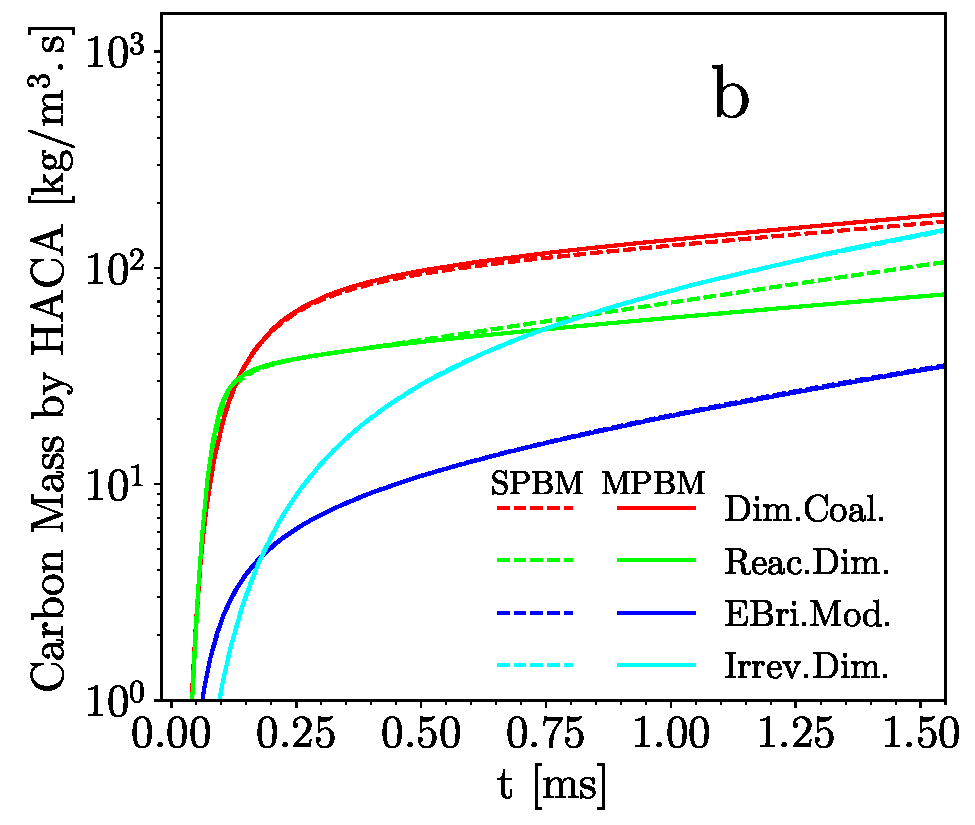
\includegraphics[width=1\textwidth]{Figures/Results/Shocktube/Stanford/June/stsh_single_HACA.pdf}
	\end{subfigure}
	\begin{subfigure}[t]{0.32\textwidth}
		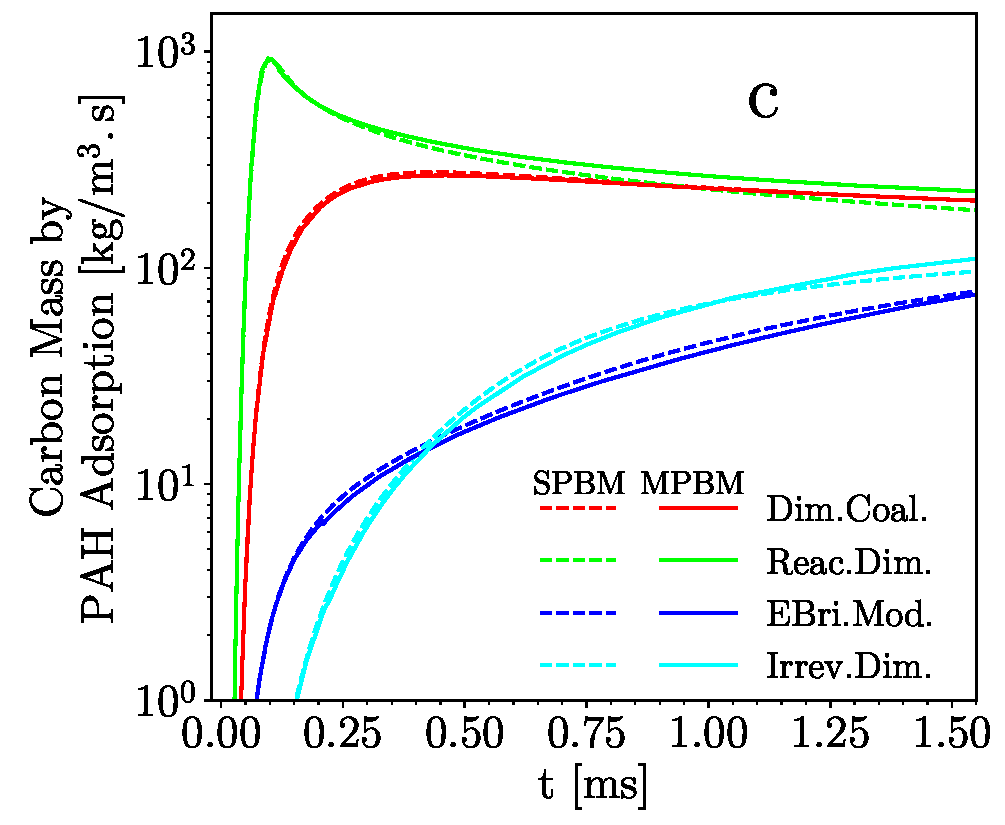
\includegraphics[width=1\textwidth]{Figures/Results/Shocktube/Stanford/June/stsh_single_PAH.pdf}
	\end{subfigure}
	\caption{The time history of carbon mass gained by inception(a), HACA (b), and PAH adsorption (c) of pyrolysis of 30\% $\mathrm{CH_4}$ at T=2455 K and P=3.47 atm using KAUST mechanism and different PAH growth and particle dynamics models}
	\label{fig:shocktubecarbon} 
\end{figure}


%----------------------------------------------------------------
%
% STANFORD SHOKCTUBE DATA 10% CH4
%
%----------------------------------------------------------------

Now, we will examine the data from Stanford's group experiments on 10\% $\mathrm{CH_4}$ pyrolysis at P=1$\pm$0.5 atm and 4$\pm$0.5 atm in the temperature range of 1900-2500 K.


\begin{table}[]
	\caption{The pressure, temperature and composition of simulation data points for 10\% $\mathrm{CH_4}$}
	\centering
	\begin{tabular}{l|llllllll|}
		\cline{2-9}
		& \multicolumn{8}{c|}{Datapoints}                       \\ \cline{2-9} 
		& (1)  & (2)  & (3)  & (4)  & (5)  & (6)  & (7)  & (8)  \\ \hline
		\multicolumn{1}{|l|}{T {[}K{]}}   & 1927 & 2074 & 2030 & 2348 & 1897 & 2085 & 2277 & 2406 \\ \hline
		\multicolumn{1}{|l|}{P {[}atm{]}} & 1.37 & 1.27 & 1.22 & 1.13 & 4.49 & 4.85 & 4.43 & 3.89 \\ \hline
		\multicolumn{1}{|l|}{Composition} & \multicolumn{8}{c|}{$\mathrm{CH_4}$: 0.1, $\mathrm{CO_2}$: 0.01, Ar: 0.7}               \\ \hline
	\end{tabular}
	\label{tab:shocktubest_CH4_10} 
\end{table}


First, the mechanism comparison is conducted by simulating 10\% $\mathrm{CH_4}$ pyrolysis in a constant volume reactor. As shown before in Figs.~\ref{fig:shocktubestch4} and ~\ref{fig:shocktubestc2h2}, the particle dynamics and PAH growth models has minimal effect on the prediction of major small hydrocarbons. So, the mechanism comparison is only based on the combination of MPBM and RD to avoid clutter in graphs, and it is focused on two data points, T=2188 K, P=1.22 atm and T=2217 K, P=4.43 atm, each being representative of atmospheric and high pressure cases, respectively. Fig.\ref{fig:shocktubes_sepch4} shows $\mathrm{CH_4}$ mole fraction for these data points predicted using KAUST, Caltech, and ABF mechanisms and compared with measurements. Similar to 30\% $\mathrm{CH_4}$ data set, KAUST and Caltech yield larger $\mathrm{CH_4}$ conversion corresponding to a lower mole fraction. However, KAUST predictions are in close agreement for both data points, but ABF underestimates $\mathrm{CH_4}$ conversion. As shown in Fig.~\ref{fig:shocktubes_sepc2h2}, all mechanisms exhibit a similar behavior underestimating $\mathrm{C_2H_2}$ mole fraction in the high pressure, but overestimating it for the atmospheric case. Fig.~\ref{fig:shocktubes_sepvf} compares soot volume fraction predicted by different mechanisms with light extinction measurements. As expected, ABF significantly underpredicts $f_v$ due to low production rate of soot precursors (PAHs). Temperature analysis is not done for 10\% $\mathrm{CH_4}$ due to lack of measurements. KAUST mechanism is used for soot analysis as it predicts species and soot volume fraction close to the measurements.

\begin{figure}[H]
	\centering
	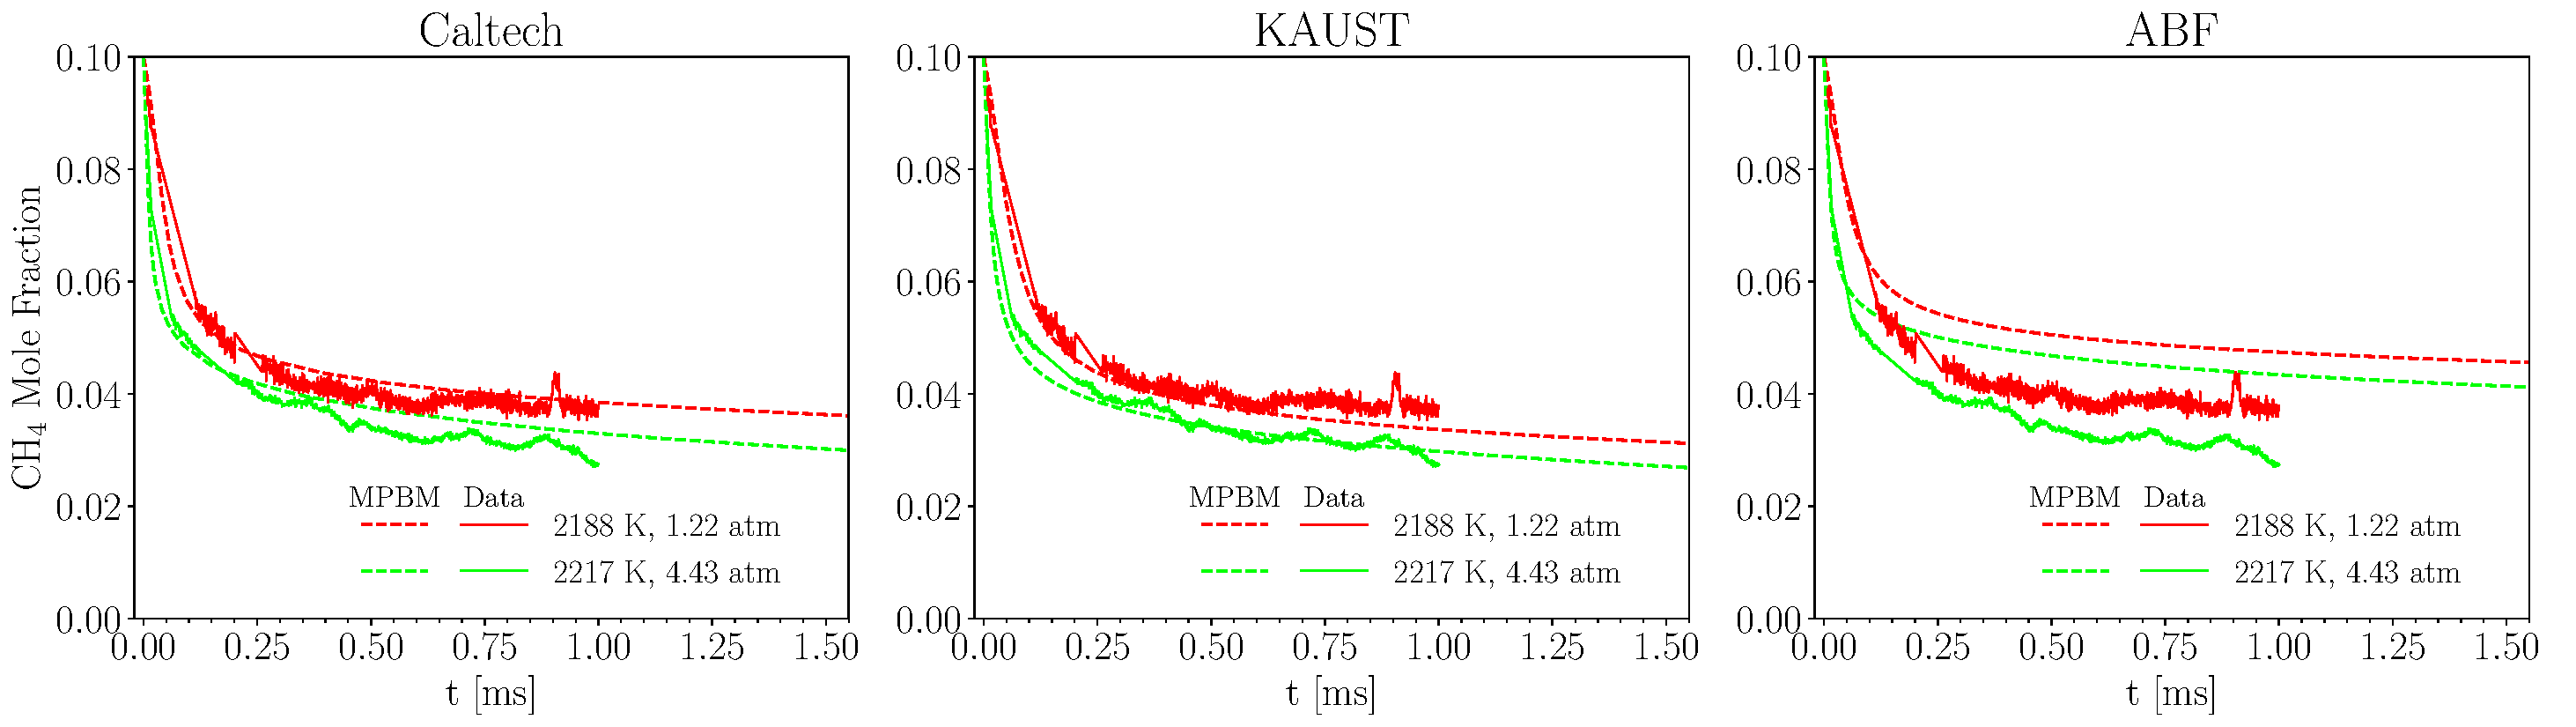
\includegraphics[width=0.9\textwidth]{Figures/Results/Shocktube/Stanford/September/stsh_sepmechs_CH4.pdf}
	\caption{The time history of $\mathrm{CH_4}$ mole fraction during 10\% $\mathrm{CH_4}$ pyrolysis at T=2188 K, P=1.22 atm (red line) and T=2217 K, P=4.43 atm (green line) using Caltech, KAUST, and ABF mechanism with MPBM and Reactive Dimerization}
	\label{fig:shocktubes_sepch4} 
\end{figure}

\begin{figure}[H]
	\centering
	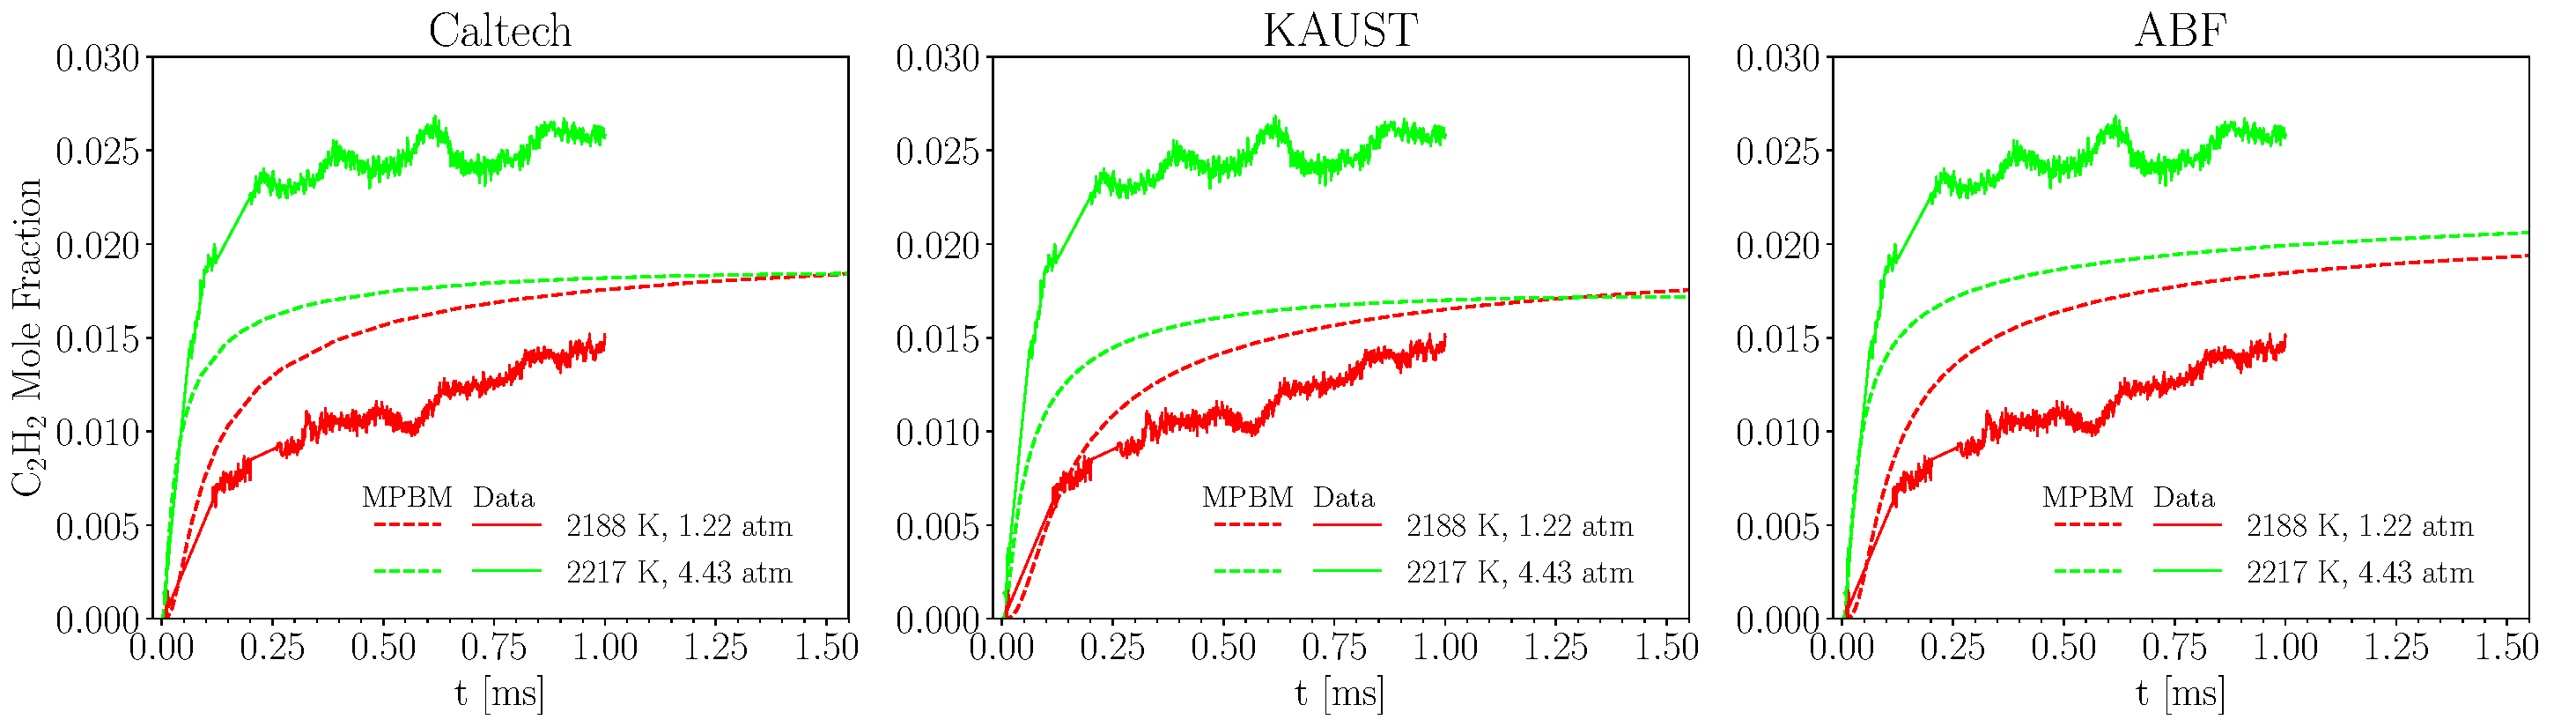
\includegraphics[width=0.9\textwidth]{Figures/Results/Shocktube/Stanford/September/stsh_sepmechs_C2H2.pdf}
	\caption{The time history of $\mathrm{C_2H_2}$ mole fraction during 10\% $\mathrm{CH_4}$ pyrolysis at T=2188 K, P=1.22 atm (red line) and T=2217 K, P=4.43 atm (green line) using Caltech, KAUST, and ABF mechanism with MPBM and Reactive Dimerization}
	\label{fig:shocktubes_sepc2h2} 
\end{figure}

\begin{figure}[H]
	\centering
	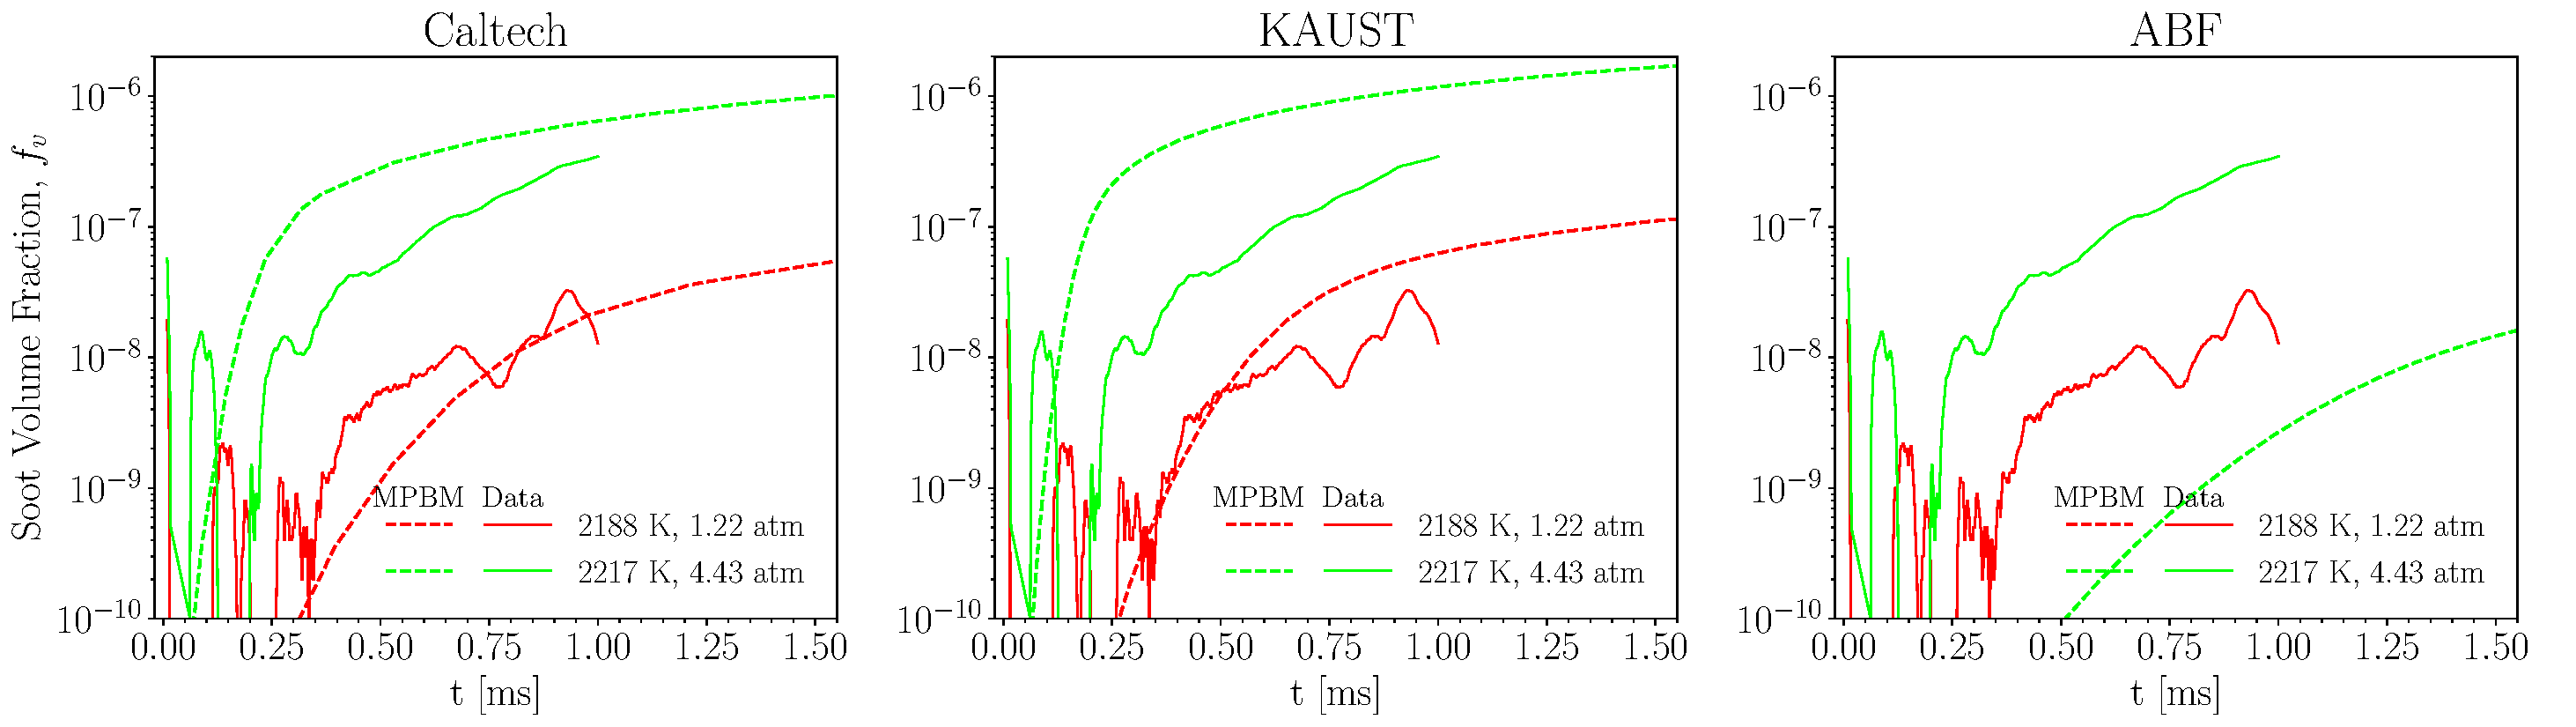
\includegraphics[width=0.9\textwidth]{Figures/Results/Shocktube/Stanford/September/stsh_sepmechs_vf.pdf}
	\caption{The time history of soot volume fraction, $f_v$ of 10\% $\mathrm{CH_4}$ pyrolysis at T=2188 K, P=1.22 atm (red line) and T=2217 K, P=4.43 atm (green line) using Caltech, KAUST, and ABF mechanism with MPBM and Reactive Dimerization}
	\label{fig:shocktubes_sepvf} 
\end{figure}

Fig.~\ref{fig:shocktubest_sepcasevf} shows the evolution of soot volume fraction, $f_v$ over simulation time in the temperature range (increasing from left to right) and (near) atmospheric and 4 atm pressure using KAUST mechanism. The upper and bottom rows correspond to 1 and 4 atm cases, and each column contains cases with similar temperatures. As expected, $f_v$ is not affected by particle dynamics model, but it increases with shock tube temperature. The time of $f_v=10^{-10}$ is shorter for 4 atm cases in each temperature indicating that pressure accelerates the soot formation. EF yields the most accurate $f_v$ prediction compared with the data in 2000-2500 K of 4 atm cases. The final $f_v$ predicted by increases by two orders of magnitude in 1900-2500 range at both pressures indicating more sensitivity of its inception rate to temperature.


\begin{figure}[H]
	\centering
	\includegraphics[width=1\textwidth]{Figures/Results/Shocktube/Stanford/September/stsh_cases_vf.pdf}
	\caption{The time history of soot volume fraction of 10\% $\mathrm{CH_4}$ pyrolysis in the temperature range of 1900-2500 K (increasing from left to right) and P=1$\pm$0.5 (bottom row) and 4$\pm$0.5 atm (upper row) using KAUST mechanism and different PAH growth and particle dynamics models}
	\label{fig:shocktubest_sepcasevf} 
\end{figure}

Figs.~\ref{fig:shocktubest_sepcasedp} and \ref{fig:shocktubest_sepcasedm} show time history of $d_p$ and $d_m$, respectively. The largest $d_p$ is predicted by RD in all cases with final values near 6 nm, which is close to $d_p$ of 10\% $\mathrm{CH_4}$. However, $d_m$ significantly decreased when feed-stock mole fraction is lowered from \%30 to \%10. Overall, the $d_p$ increases slightly with both temperature and pressure. RD has the largest $d_m$ in the entire temperature range of atmospheric cases, but at 4 atm $d_m$ by DC quickly increases and exceed RD due to stronger inception rate leading to larger coagulation rate and agglomerates. 

\begin{figure}[H]
	\centering
	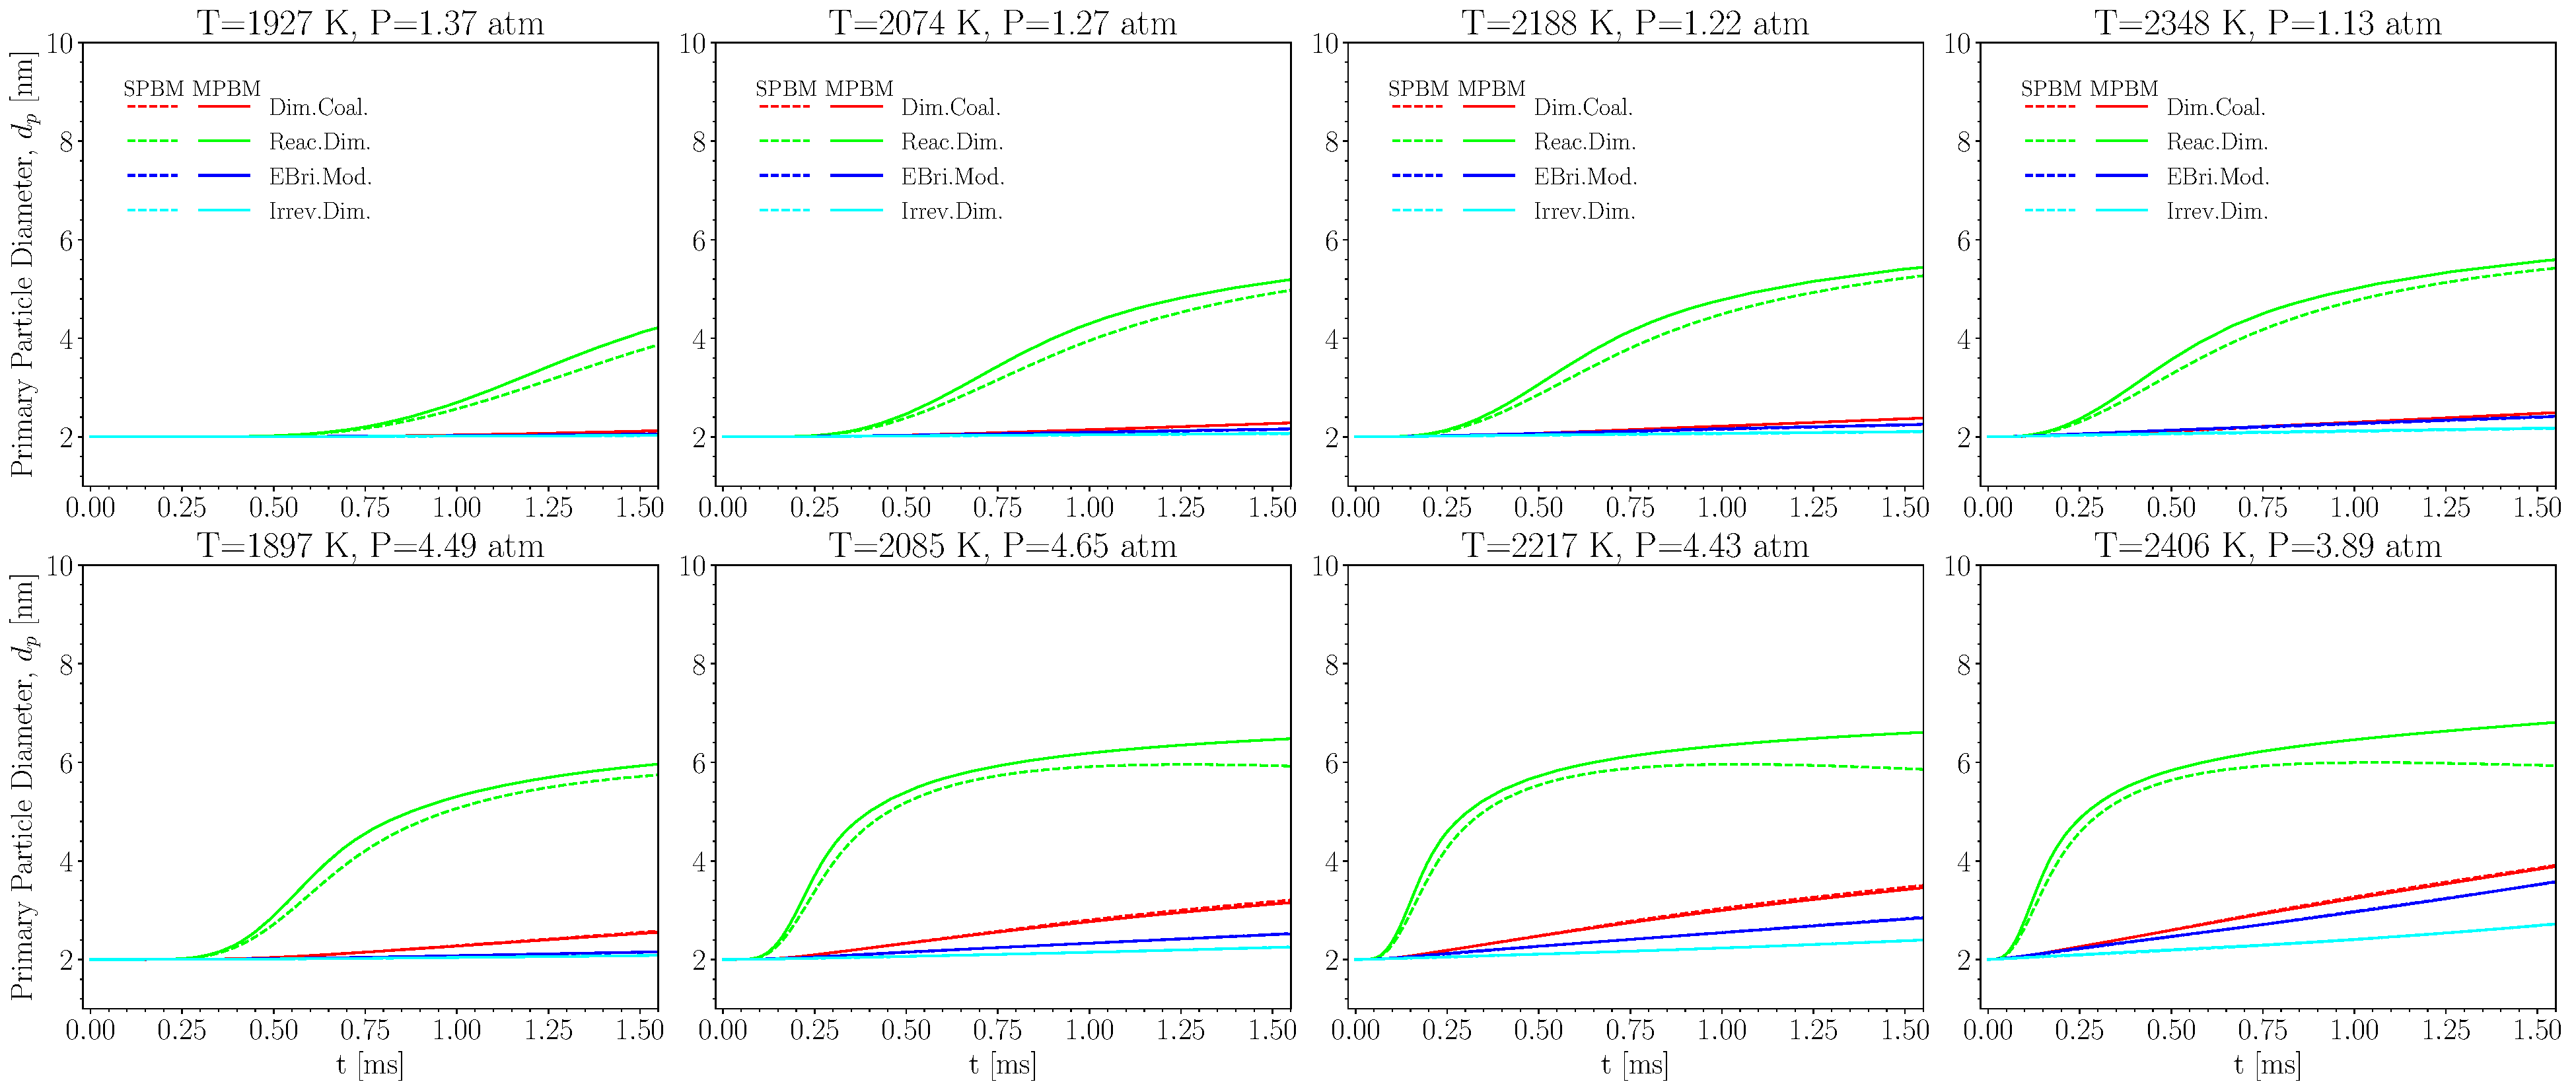
\includegraphics[width=1\textwidth]{Figures/Results/Shocktube/Stanford/june/stsh_cases_dp.pdf}
	\caption{The time history of primary particle diameter, $d_p$ of 30\% $\mathrm{CH_4}$ pyrolysis in the temperature range of 1800-2500 K and P=1$\pm$0.5 and 4$\pm$0.5 atm using KAUST mechanism and different PAH growth and particle dynamics models}
	\label{fig:shocktubest_sepcasedp} 
\end{figure}

\begin{figure}[H]
	\centering
	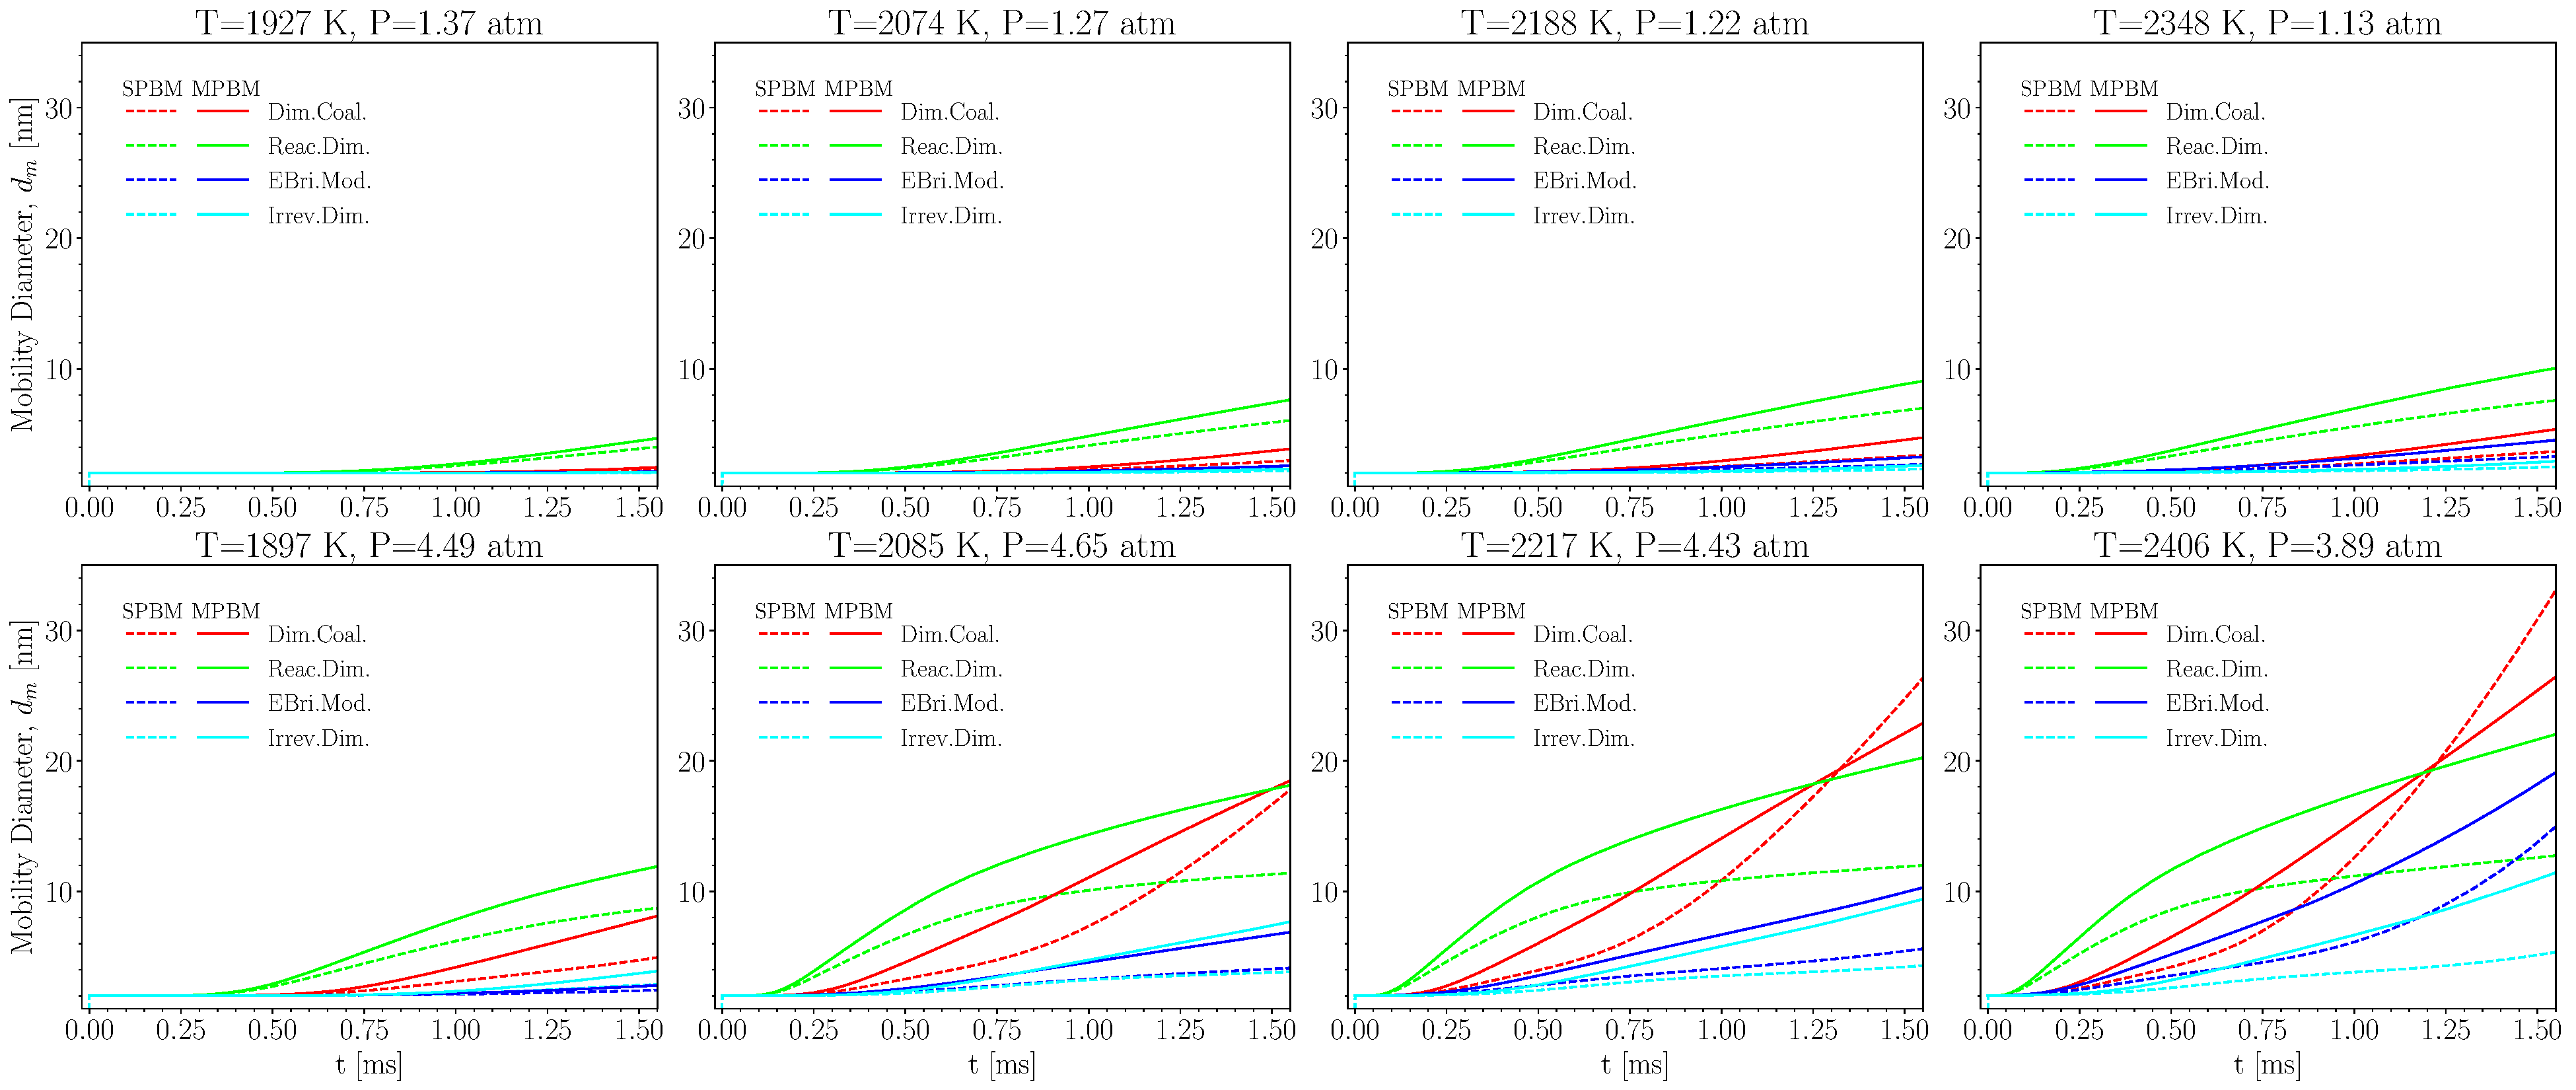
\includegraphics[width=1\textwidth]{Figures/Results/Shocktube/Stanford/September/stsh_cases_dm.pdf}
	\caption{The time history of mobility diameter, $d_m$ of 30\% $\mathrm{CH_4}$ pyrolysis in the temperature range of 1800-2500 K and P=1$\pm$0.5 and 4$\pm$0.5 atm using KAUST mechanism and different PAH growth and particle dynamics models}
	\label{fig:shocktubest_sepcasedm} 
\end{figure}

\subsection{Analysis of soot morphology in methane pyrolysis shock-tube}

The TEM images of 10\% $\mathrm{CH_4}$ at T=2230 K and P=4.5 atm data point provided by Stanford group are used to evaluate the performance of omnisoot in the prediction of $\mathrm{d_p}$ and $\mathrm{d_m}$ and compare the effect of different PAH growth and particle dynamics model on morphology. Soot particles are sampled from \hl{the end pipe wall} and analyzed using a \hl{****} Transmission Electron Microscopy model \hl{****} over \hl{****} TEM grid. As reported by Stanford team, the expansion wave traverses the shock tube around 2 ms reducing the temperature to nearly \hl{****} K freezing the chemical reactions that contribute to the surface growth, but the coagulation might continue until the collection of particles leading to larger agglomerates. As a result, $d_p$ estimated from the TEM images closely represents $d_p$ of agglomerates at the end of process, but TEM-based $d_m$ could be larger the actual values due to post expansion wave growth of particles. \textit{atems} package~\citep{sipkens2021using} was used for characterizing soot aggregates in TEM images with different methods for evaluating the aggregate projected area, perimeter, and primary particle diameter. It creates a binary map from the raw TEM image where white and black pixels represent the agglomerates and background, respectively, and feeds the map to a agglomerate segmentation algorithm to detect individual agglomerates. Fig.\ref{fig:shocktubest_binarymapprocess} shows a sample from TEM images and segmented agglomerates from generated map.

\begin{figure}[H]
	\centering
	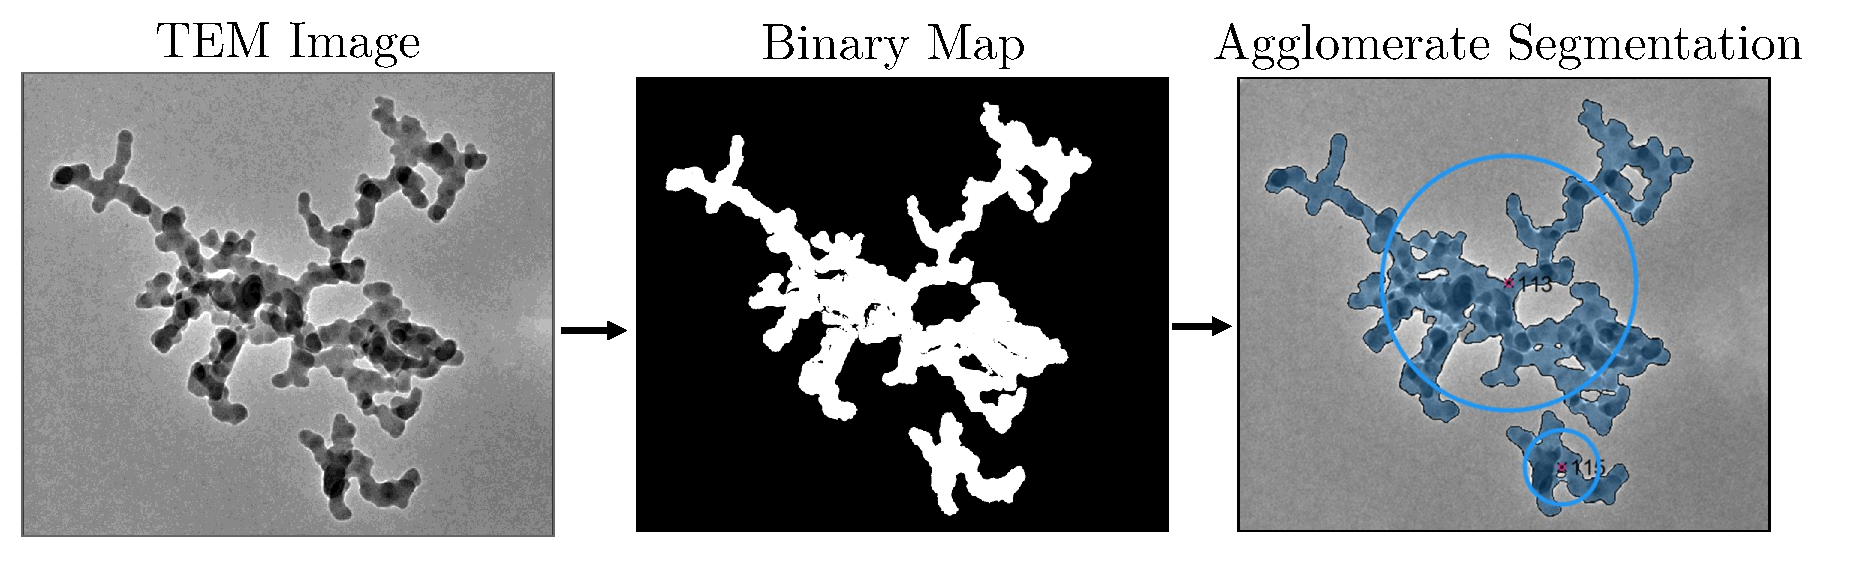
\includegraphics[width=0.9\textwidth]{Figures/Results/Shocktube/Stanford/TEM/binarymapprocess.pdf}
	\caption{A TEM image provided by Stanford group (left pane) with the generated binary map (middle pane) and detected agglomerates using the segmentation algorithm (right pane)}
	\label{fig:shocktubest_binarymapprocess} 
\end{figure}

We applied K-means clustering (KMC)~\citep{sipkens2021using} and otsu thresholding~\citep{dastanpour2016automated} to the same TEM images and compared the segmented agglomerates. A sample is shown in Fig.\ref{fig:shocktubest_aggseg_compare} where  KMC detected more agglomerates in the TEM image, but segments part of the background as agglomerates or divides a single agglomerate into multiple ones. On the other hand, otsu thresholding misses most of agglomerates in the TEM image. Here, the  K-means clustering~\citep{sipkens2021using} is used and 171 agglomerates were detected. $d_m$ was calculated from the diameter of equivalent projected area , $A_a$ of each agglomerate. The pair correlation method (PCM)~\citep{dastanpour2016automated} was applied to compute the projected primary particle area, $A_p$ and the mean $d_p$ assuming that primary particle are almost uniform in size within each agglomerate. The number of primary particle per agglomerate is calculated as $n_p=A_a/A_p$ resulting in 6554 primary particles. The mean $d_p$ of the entire samples is calculated as 

\begin{equation}
	\overline{d}_{p} = \frac{\sum_{Aggs} n_p d_p}{\sum_{Aggs} n_p} 
	\label{eqn:meandp}
\end{equation}


\begin{figure}[H]
	\centering
	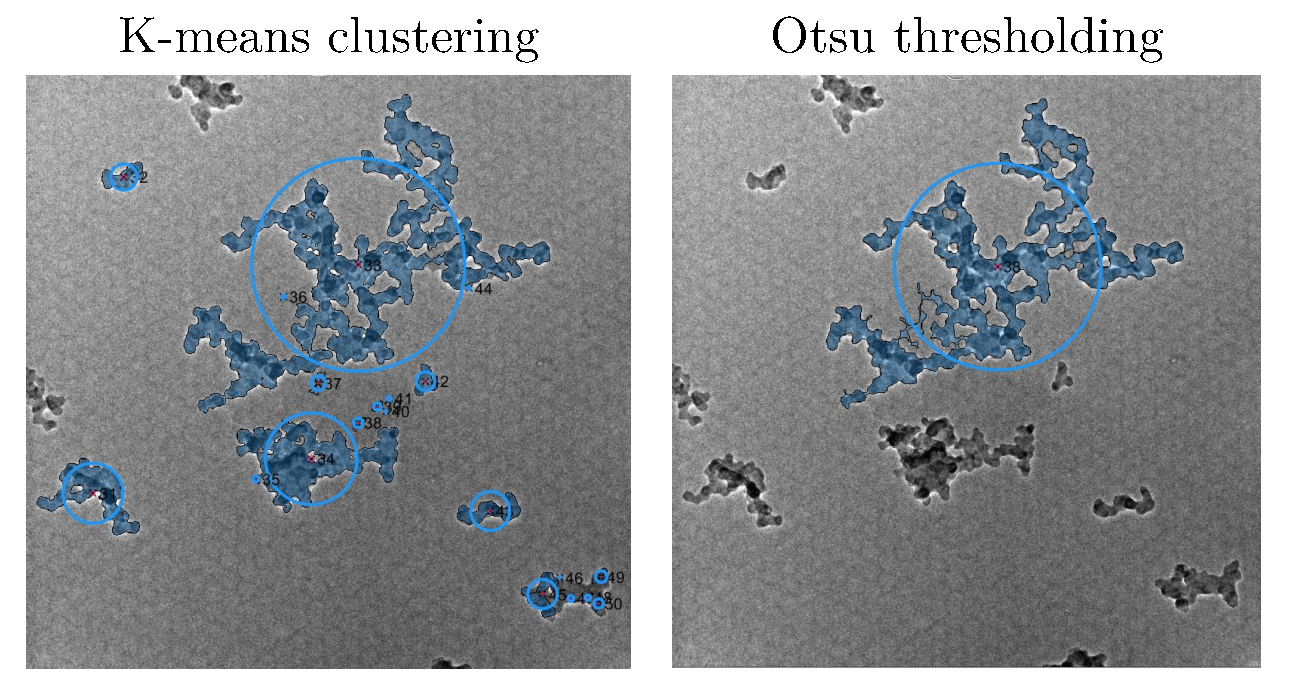
\includegraphics[width=0.6\textwidth]{Figures/Results/Shocktube/Stanford/TEM/aggseg_compare.pdf}
	\caption{Agglomerates in single TEM image segmented by K-means clustering (left pane) and otsu thresholding (right pane)}
	\label{fig:shocktubest_aggseg_compare} 
\end{figure}


\begin{table}
	\caption{The morphological characteristics of agglomerates quantified by atems using KMC and PCM}
	\label{tab:shocktube_TEM_morph}
	\centering
	\begin{tabular}{l l l}
		\hline
		Property & Arithmetic mean & Median \\
		\hline
		$d_m$ [nm] & 97 & 69 \\
		$d_p$ [nm] & 22 & 18 \\
		\hline
	\end{tabular}
\end{table}


Table~\ref{fig:shocktubest_aggseg_compare} reports the arithmetic mean and median of mobility and primary particle diameter detected by atems from TEM images. The computed $d_m$ and $d_p$ will be compared with soot sampled from various sources. Soot morphology is mainly governed by coagulation leading to self-similar structures in which $d_m$ scales with $d_p$ and $n_p$. 
%Following that principle, a power-law derived from DEM simulation in flame conditions~\citep{Kelesidis2017} was introduced in Sec.~\ref{sec:sootmorphology}. Here, we compare the ratio of mobility to primary particle diameter $d_m/d_p$ with $d_m/d_p=n_p^{0.45}$ (Eq.~\ref{eqn:d_m}). 
\citet{olfert2019universal} analyzed soot particles from flares~\citep{kazemimanesh2019size}, inverted burners~\citep{dastanpour2017variation}, compression ignition engines~\citep{graves2015characterization} and other sources to support the external mixing hypothesis and related agglomerate size characterized by $d_m$ to $d_p$ using the following power-law:

\begin{equation}
	d_{p} = d_{p,100} 
	\left(
	\frac{d_m}{100 nm}
	\right)^{D_{\mathrm{TEM}}},
	\label{eqn:usf}
\end{equation}

\noindent where $d_{p,100}$ is the average primary particle diameter for a 100 nm aggregate, and $D_{\mathrm{TEM}}$ is the exponent. Both quantities were obtained by fitting Eq.~\eqref{eqn:usf} to soot sampled from different sources. the left pane of Fig~\ref{fig:shocktube_TEM_powerlaws} demonstrates the scatter plot of $d_p$ against $d_m$ is compared with power-law curves of Eq.~\eqref{eqn:usf} using two sets of prefactor and exponent values, i) $D_{\mathrm{TEM}}$=0.32, $d_{\mathrm{p,100}}$=20.6 nm, and ii) $D_{\mathrm{TEM}}$=0.39, $d_{\mathrm{p,100}}$=20.2 nm taken from average values reported in summary of fit parameters in Table 1 of \citet{olfert2019universal}. The power-law show a good agreement with quantities that $d_p$ and $d_m$ computed by atems can be good representative of soot agglomerates with minimal agglomerate overlap.

\begin{figure}[H]
	\centering
	\begin{subfigure}[t]{0.32\textwidth}
		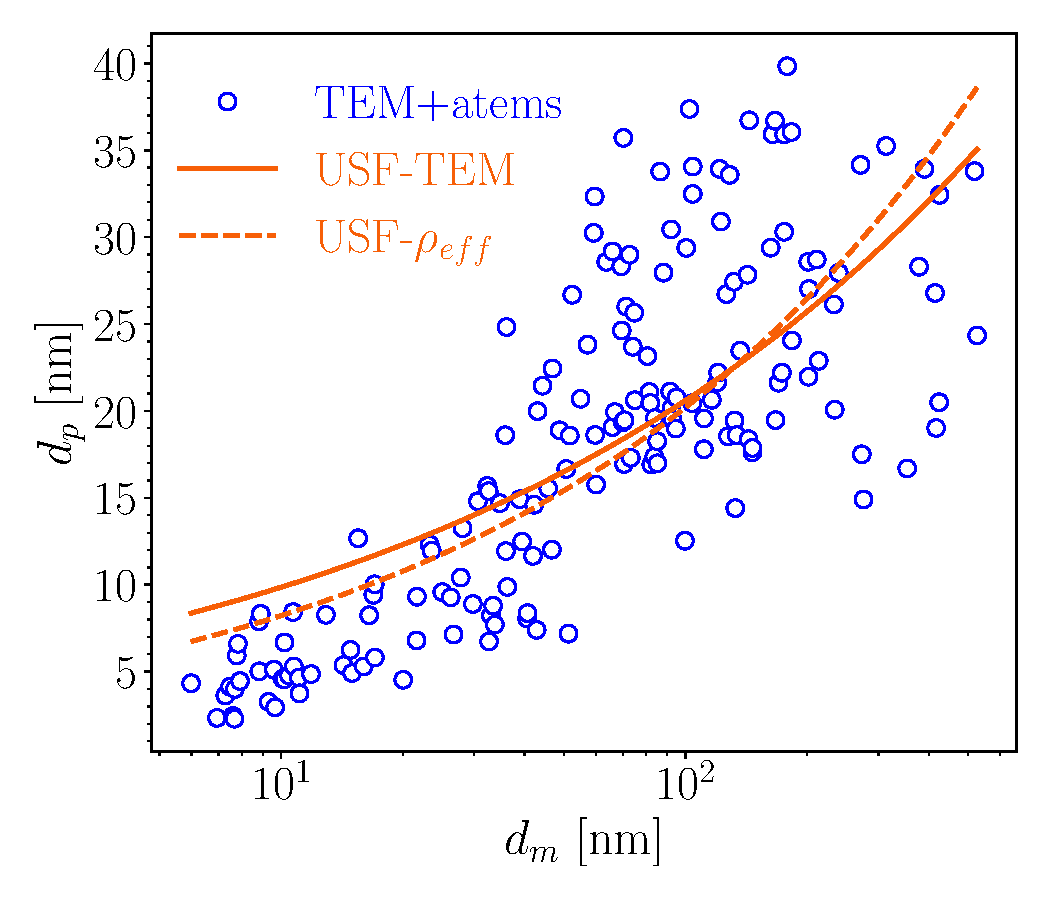
\includegraphics[width=1\textwidth]{Figures/Results/Shocktube/Stanford/TEM/dmdp_scalelaw.pdf}
	\end{subfigure}
	\caption{The $d_m$ as a function of $d_p$ from TEM image obtained by atems~\citep{sipkens2021using} (symbols) compared with the power law in Eq.~\eqref{eqn:usf}} 
	\label{fig:shocktube_TEM_powerlaws} 
\end{figure}

Fig.~\ref{fig:shocktube_TEM_fvdd} compares $f_v$ from extinction measurement, $d_p$ and $d_m$ computed from TEM images with model predictions using KAUST mechanism, Monodisperse and different PAH growth models. The horizontal error bars denotes the uncertainty in residence time that TEM measurements correspond to. As reported by Stanford group, the expansion wave propagates near t=2 ms stopping the growth of $d_p$. Although the predicted soot mass, represented by volume fraction, is close even greater than measurements, but $d_p$ is underpredicted by all PAH growth models. RD yields the largest $d_p$ near 7 nm that is lower than $d_p$ from TEM measurements by a factor of 3.

\begin{figure}[H]
	\centering
	\begin{subfigure}[t]{0.3\textwidth}
		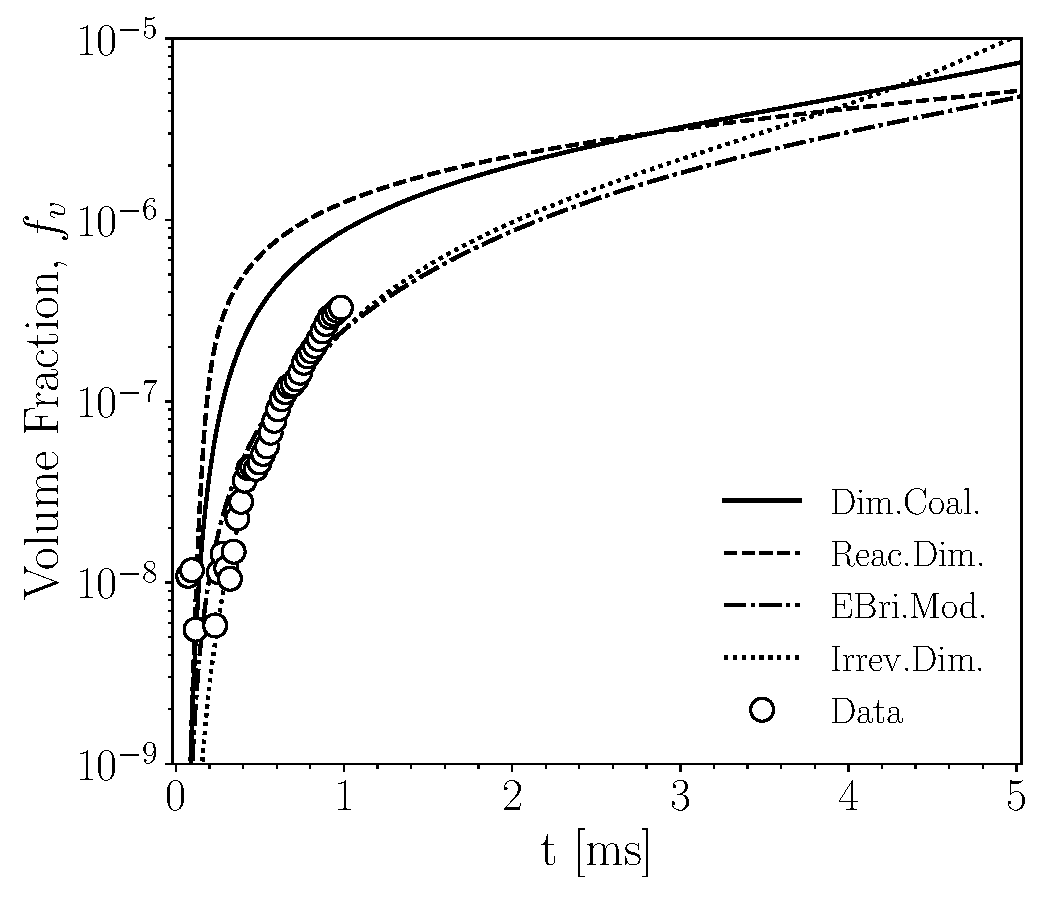
\includegraphics[width=1\textwidth]{Figures/Results/Shocktube/Stanford/TEM/vf_TEM.pdf}
	\end{subfigure}
	\begin{subfigure}[t]{0.32\textwidth}
		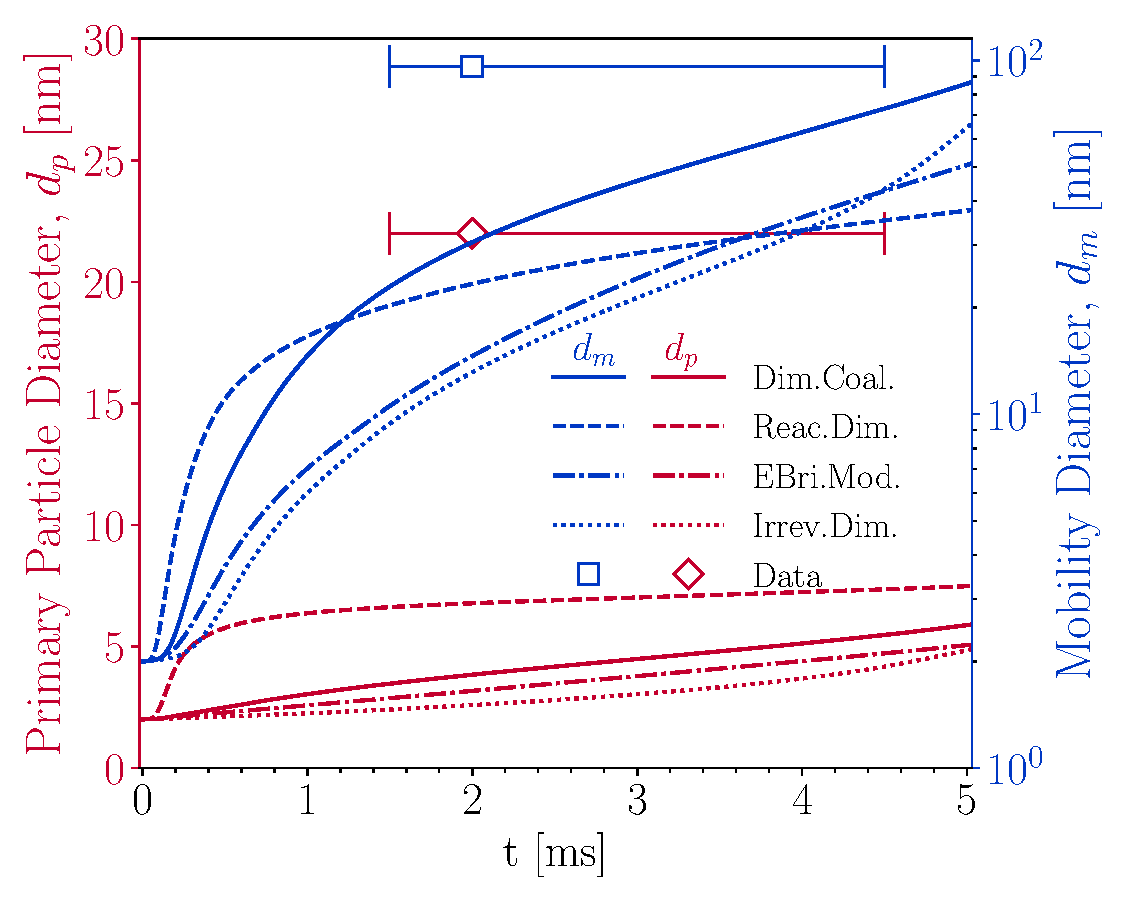
\includegraphics[width=1\textwidth]{Figures/Results/Shocktube/Stanford/TEM/dp_dm_TEM.pdf}
	\end{subfigure}
	\caption{The volume fraction, $f_v$ (left pane) and mobility, $d_m$ (blue lines in right pane) and primary particle diameter, $d_p$ (red lines in right pane) predicted by KAUST mechanism, MPBM, and different PAH growth models at T=2230 K, P=4.5 atm that corresponds to shock-tube conditions of TEM measurement}
	\label{fig:shocktube_TEM_fvdd} 
\end{figure}

\subsection{Sensitivity of yield and morphology to inception and surface growth rate}

The underprediction of $d_p$ by the model despite producing enough or even more soot carbon mass compared with the measurement motivated performing a sensitivity analysis for soot yield and morphology, especially because of uncertainties in inception and surface growth pathways and reaction rates associated with the PAH growth models integrated in omnisoot. It should be noted that this section is not aimed at a systematic sensitivity analysis with respect to all reaction rates, but rather to determine which sub-model has the dominant effect on yield and morphology that can be modified within the physical constraints to tailor these quantities to the desired values.

First, we examine the effect of HACA rates on yield and morphology of soot generated during 10\% $\mathrm{CH_4}$ at T=2230 K and P=4.5 atm in the Stanford shock-tube. To this  purpose, the surface reactivity, $\alpha$, in HACA formulation is modified by introducing a damping factor, $\zeta$ in Eq.~\eqref{eqn:hacaRate} as:

\begin{equation}
	\alpha^i = \tanh 
	\left(
	\frac{12.56 - 0.00563\cdot \zeta T}
	{\mbox{log}_{10}
		\left( \frac{\rho_{soot}\cdot Av}{W_{carbon}} \frac{\pi}{6}{d^i_p}^3 \right) } -1.38+0.00068\cdot \zeta T
	\right)
	\label{eqn:alpha_modified}.
\end{equation}

Note that, there are many adjustable parameters in HACA scheme such as rate constants. $\zeta$ to modify $\alpha$ is intentionally chosen for a number of reasons. First, $\alpha$ was initially introduced as a tuning parameter as a function of local temperature and primary particle diameter to control surface growth rate, and it has been usually adjusted specifically for each flame~\citep{castaldi1996pah, xu1997soot} to match the predicted volume fraction with the measurements. Second, the global empirical relation of \citet{appel2000kinetic} (used omnisoot to quantify $\alpha$) developed by fitting parameters of $\alpha$ to minimize the prediction error of volume fraction for various premixed flames, and shock tubes generally have larger temperature ranges compared with premixed flames, which could excessively reduce surface reactivity and HACA growth rates. Finally, larger volume fractions (in the order of few ppm) were underpredicted by the global $\alpha$ relation (Fig. 9 of \citep{appel2000kinetic}). So, the low values of $\alpha$ in the shock tube at T=2230 K corresponding to process conditions of TEM measurements can contribute to underprediction of surface growth rates and $d_p$. We introduce $\zeta$ to reduce the damping effect of temperature on surface reactivity. Fig.~\ref{fig:shocktube_alpha_HACA} demonstrates the variation of $\alpha$ with temperature for $\zeta$=0.6, 0.8, 1 and primary particle diameter 2 and 6 nm. $\alpha$ decreases with temperature, and it is inversely proportional to $\zeta$. 

\begin{figure}[H]
	\centering
	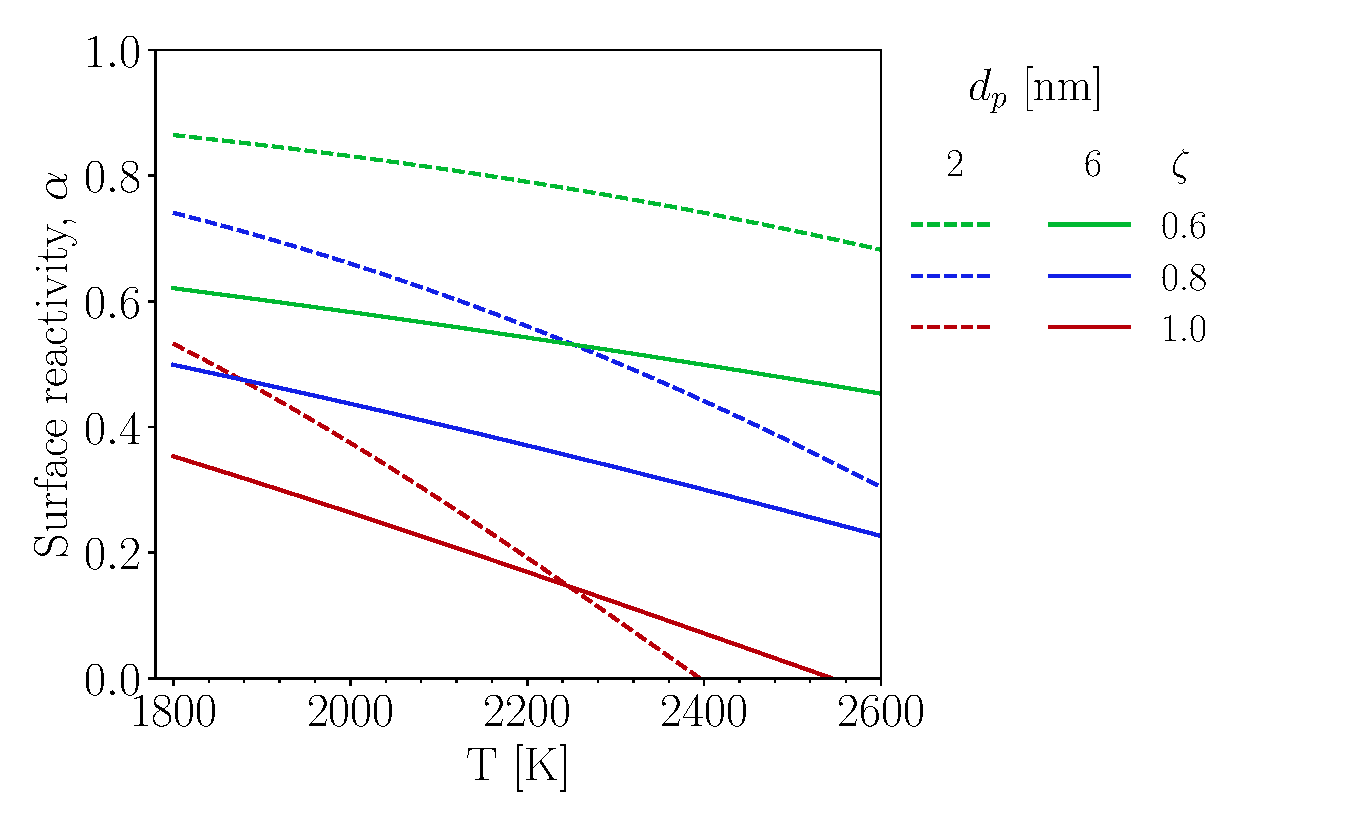
\includegraphics[width=0.5\textwidth]{Figures/Results/Shocktube/HACA/alpha.pdf}
	\caption{The variation of surface reactivity, $\alpha$, as a function of temperature for different values of $\zeta$ and primary particle size of 2 nm (dashed lines) and 6 nm (solid lines)}
	\label{fig:shocktube_alpha_HACA} 
\end{figure}

A series of simulation were performed to study the damping effect of temperature on soot mass and morphology by varying   $\zeta$ from 1 to 0.8 and 0.6. Note that, $\zeta$ of 1 represent the original $\alpha$ formulation. The reaction mechanism and particle dynamic model were set to KAUST and MPBM, respectively, but all PAH growth were used in the simulations.
Fig.~\ref{fig:shocktube_vf_zetseffect} and~\ref{fig:shocktube_sy_zetseffect} depicts the volume fraction and soot carbon yield, respectively. As expected, both quantities increases by reducing $\zeta$. The difference due to three $zeta$ values become significant only after t=1.5 ms, so it does not change the agreement with measurements available up to 1 ms. The final SY at the end of 5 ms increases by a factor of 1.3 to 2 depending on the PAH growth model by varying $\zeta$ from 1 to 0.6. Additionally, soot yield for DC, EF, and ID models levels off towards the end of simulation indicting the maximum yield.

\begin{figure}[H]
	\centering
	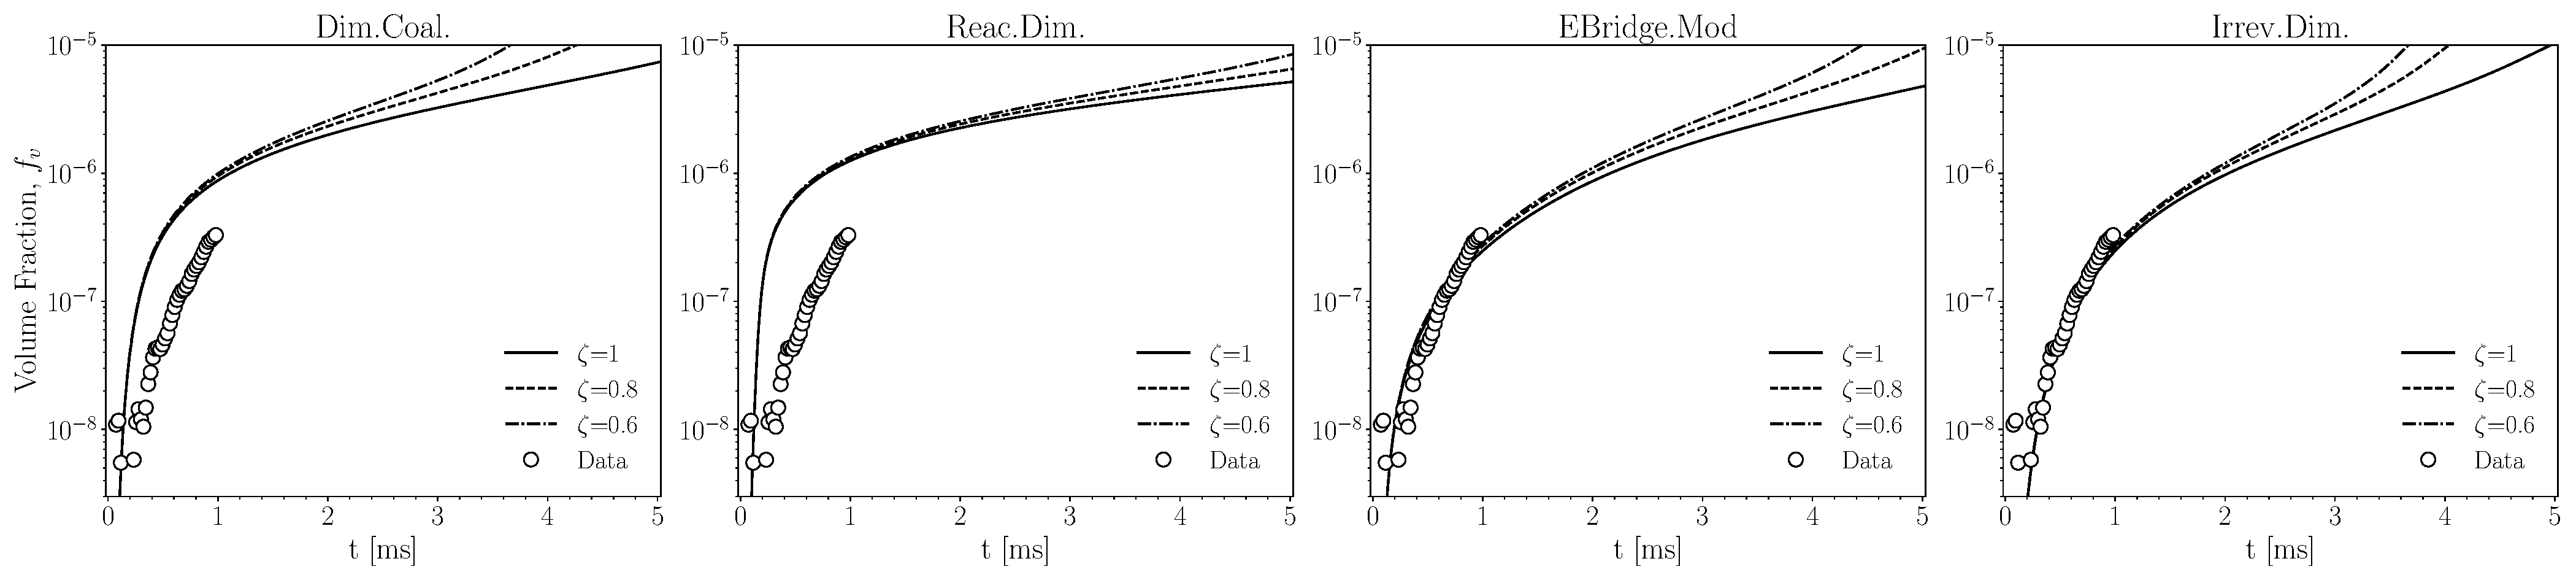
\includegraphics[width=1\textwidth]{Figures/Results/Shocktube/Stanford/TEM/vf_all_zetaeffect.pdf}
	\caption{The effect of reducing $\zeta$ leading to larger HACA rates on soot volume fraction, $f_v$ using KAUST and MPBM and different PAH growth model}
	\label{fig:shocktube_vf_zetseffect} 
\end{figure}


\begin{figure}[H]
	\centering
	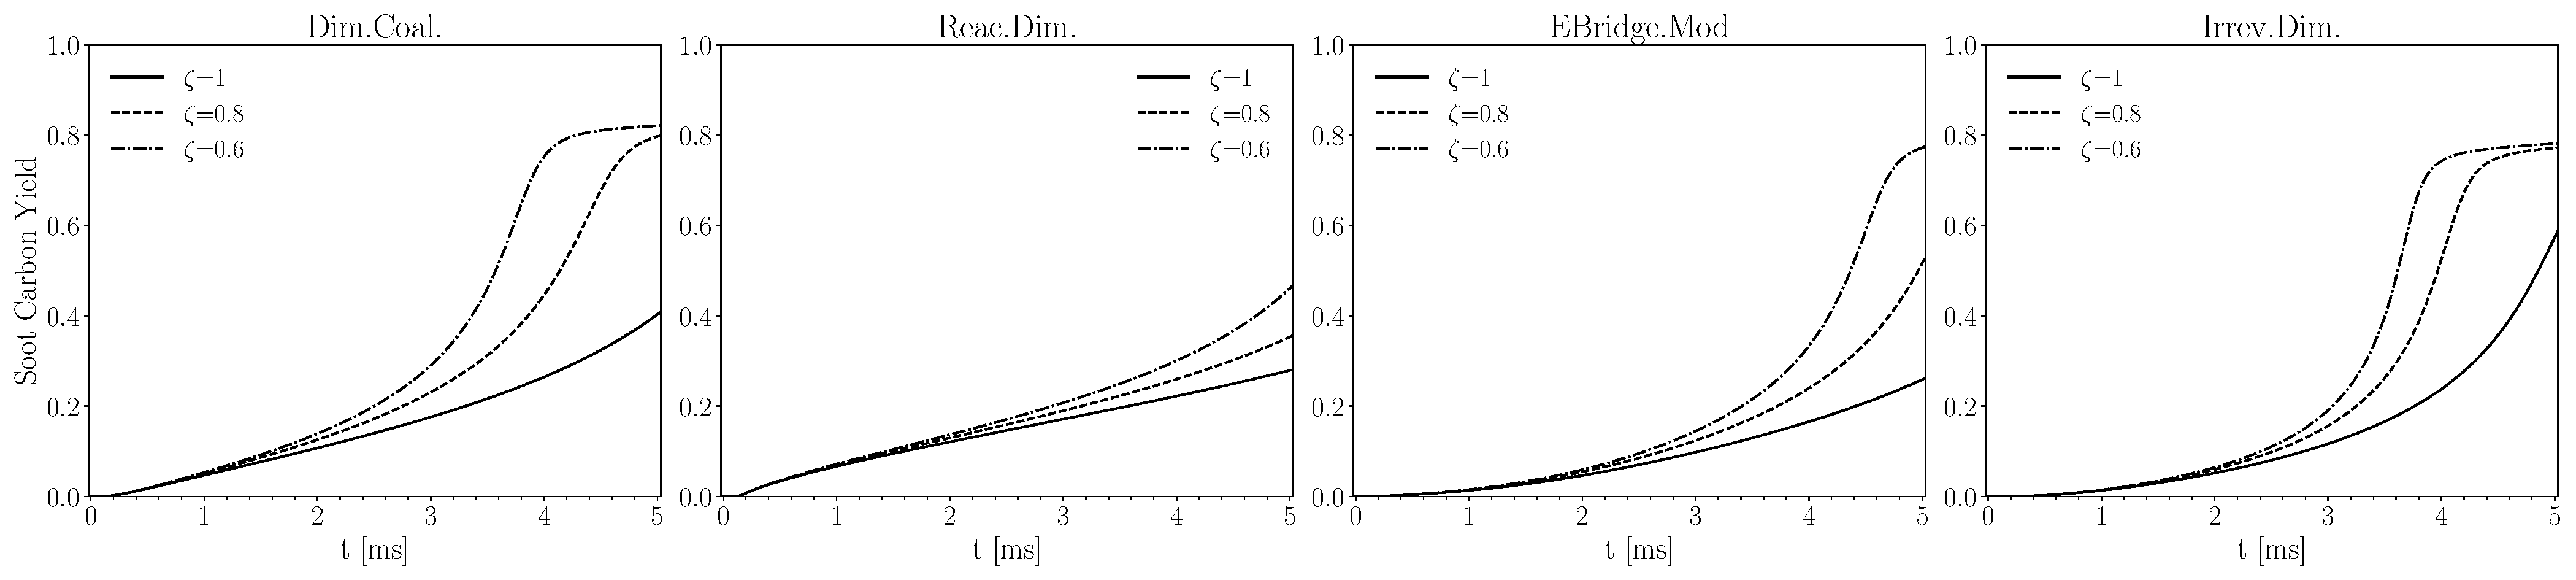
\includegraphics[width=1\textwidth]{Figures/Results/Shocktube/Stanford/TEM/sy_all_zetaeffect.pdf}
	\caption{The effect of reducing $\zeta$ leading to larger HACA rates on soot carbon yield using KAUST and MPBM and different PAH growth model}
	\label{fig:shocktube_sy_zetseffect} 
\end{figure}

Fig.\ref{fig:shocktube_ddd_zetseffect} demonstrates changes of $d_p$ and $d_m$ due to $\zeta$ values using different PAH growth models. Reducing $\zeta$ to 0.6 increases $d_p$ to a maximum of 2 nm. $d_p$ predicted by DC, EF, and ID model reaches its maximum indicating that smaller $\zeta$ values (higher HACA rate) will not change the maximum $d_p$. The simulations using different $\zeta$ values highlight relatively low sensitivity of $d_p$ with respect to surface reactivity in 10\% $\mathrm{CH_4}$ pyrolysis in shock tube described using a constant volume reactor.

\begin{figure}[H]
	\centering
	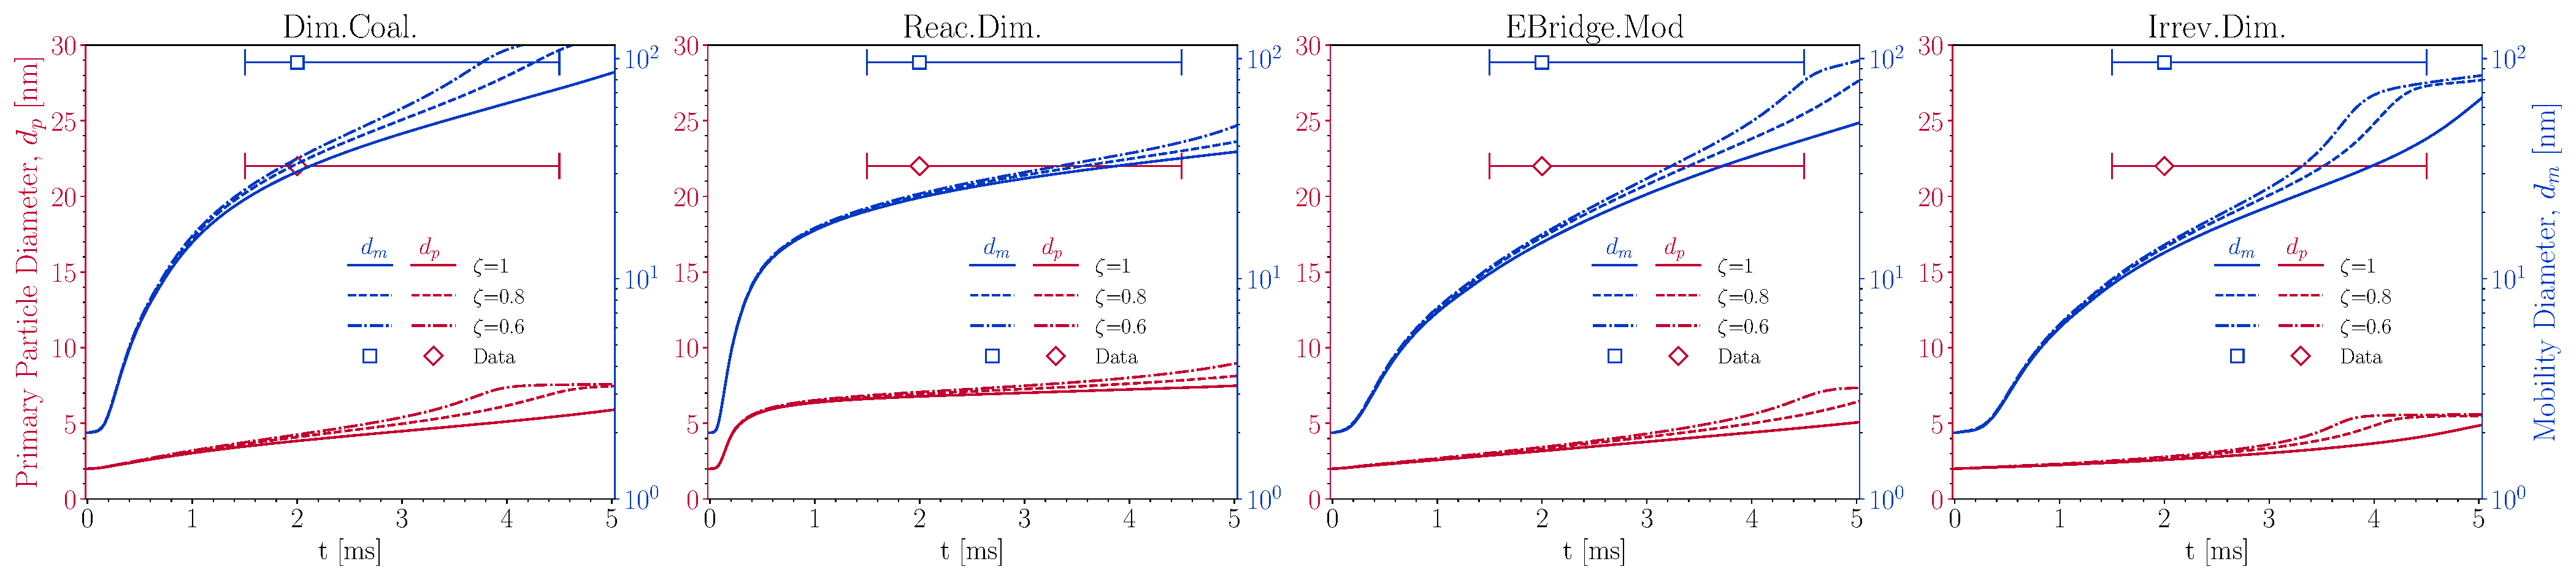
\includegraphics[width=1\textwidth]{Figures/Results/Shocktube/Stanford/TEM/dp_dm_zetaeffect.pdf}
	\caption{The effect of reducing $\zeta$ leading to larger HACA rates on mobility, $d_m$ and primary particle diameter, $d_p$ using KAUST and MPBM and different PAH growth model}
	\label{fig:shocktube_ddd_zetseffect} 
\end{figure}